\begin{frame}
\end{frame}

\begin{frame}{Large Networks, Large Datasets}
\protect\hypertarget{large-networks-large-datasets}{}
\begin{itemize}
\tightlist
\item
  Training models that solve complex, real world tasks requires large
  model and data scale
\end{itemize}

\vspace{-0.2cm}
\center{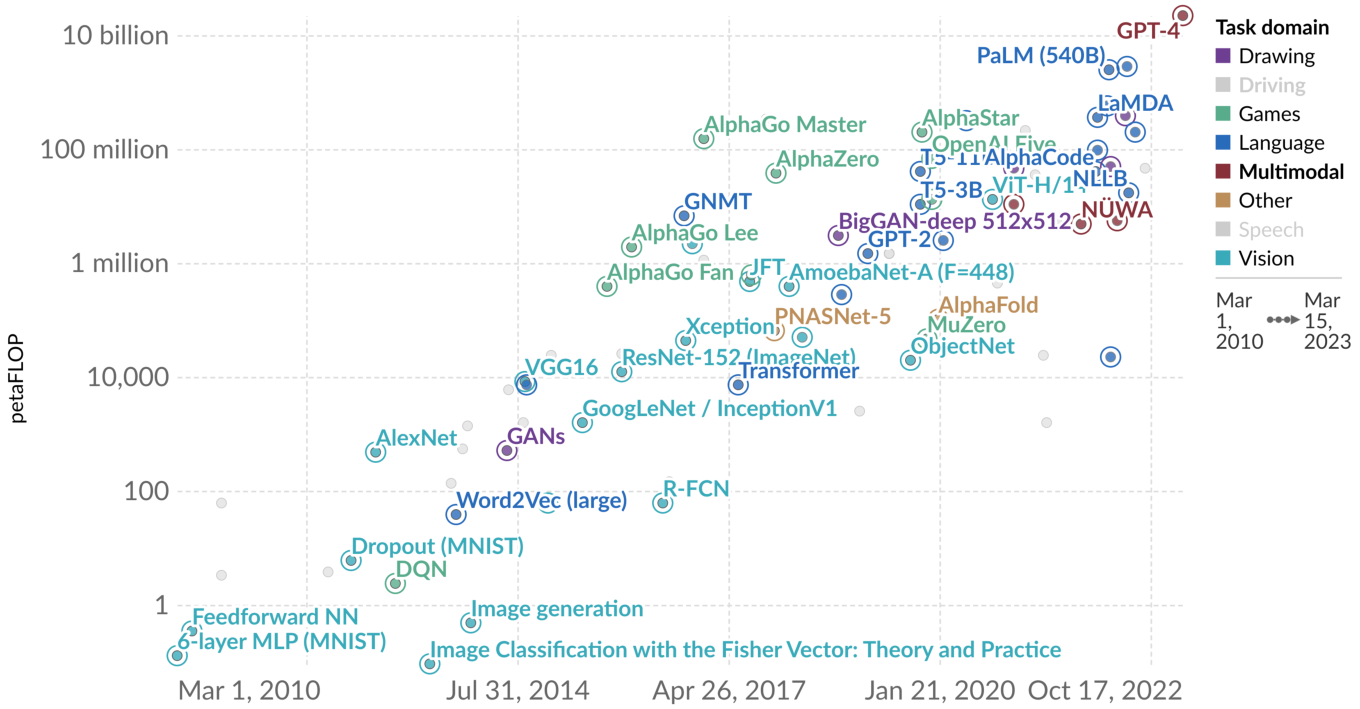
\includegraphics[width=0.9\textwidth]{../images/Compute_Budget_Training_Milestone_models_2022_mod.pdf}}

\vspace{-0.5cm}

\footnote<.->{\tiny Sevilla et al., 2023;
  OurWorldInData.org/artificial-intelligence; CC BY Source}
\end{frame}

\begin{frame}{Large Networks, Large Datasets}
\protect\hypertarget{large-networks-large-datasets-1}{}
\begin{itemize}
\tightlist
\item
  Networks : large models, many layers, large number of parameters
  (weights)

  \begin{itemize}
  \tightlist
  \item
    Vision: Convolutional, Transformer and Hybrid networks
  \item
    hundreds of layers, hundred millions of parameters (currently up to
    20B)
  \end{itemize}
\end{itemize}

\center{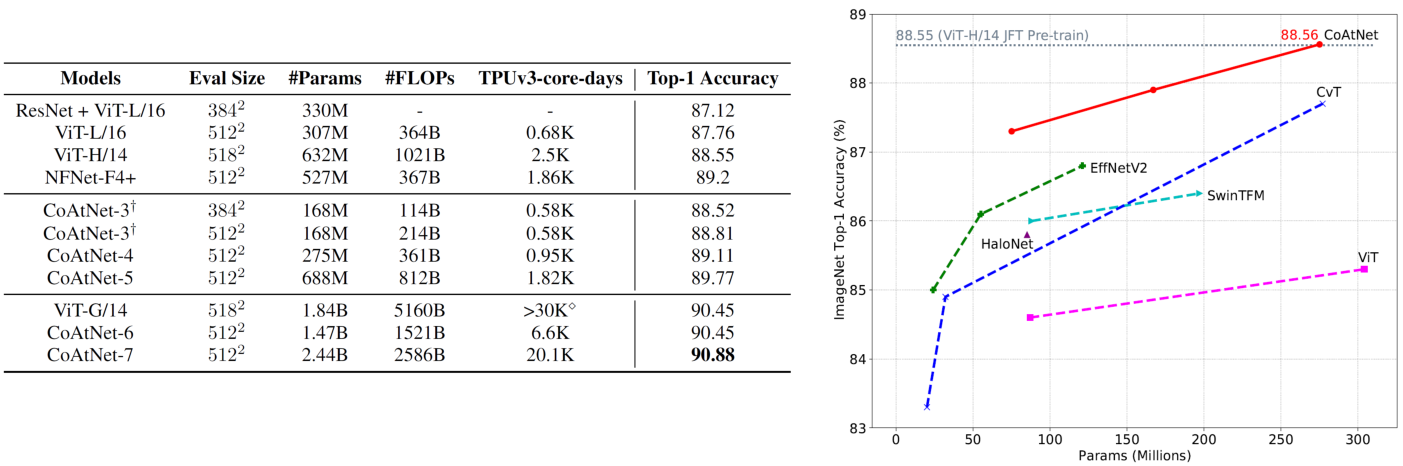
\includegraphics[width=\textwidth]{../images/Vision_Networks_CoAtNet_2021_mod.pdf}}

\footnote<.->{\tiny Dai et al, NeurIPS, 2021}
\end{frame}

\begin{frame}{Large Networks, Large Datasets}
\protect\hypertarget{large-networks-large-datasets-2}{}
\begin{itemize}
\tightlist
\item
  Networks : large models, many layers, large number of parameters
  (weights)

  \begin{itemize}
  \tightlist
  \item
    Language: Transformer networks
  \item
    hundreds of layers, billions of parameters (GPT-3: 175 Billion)
  \end{itemize}
\end{itemize}

\center{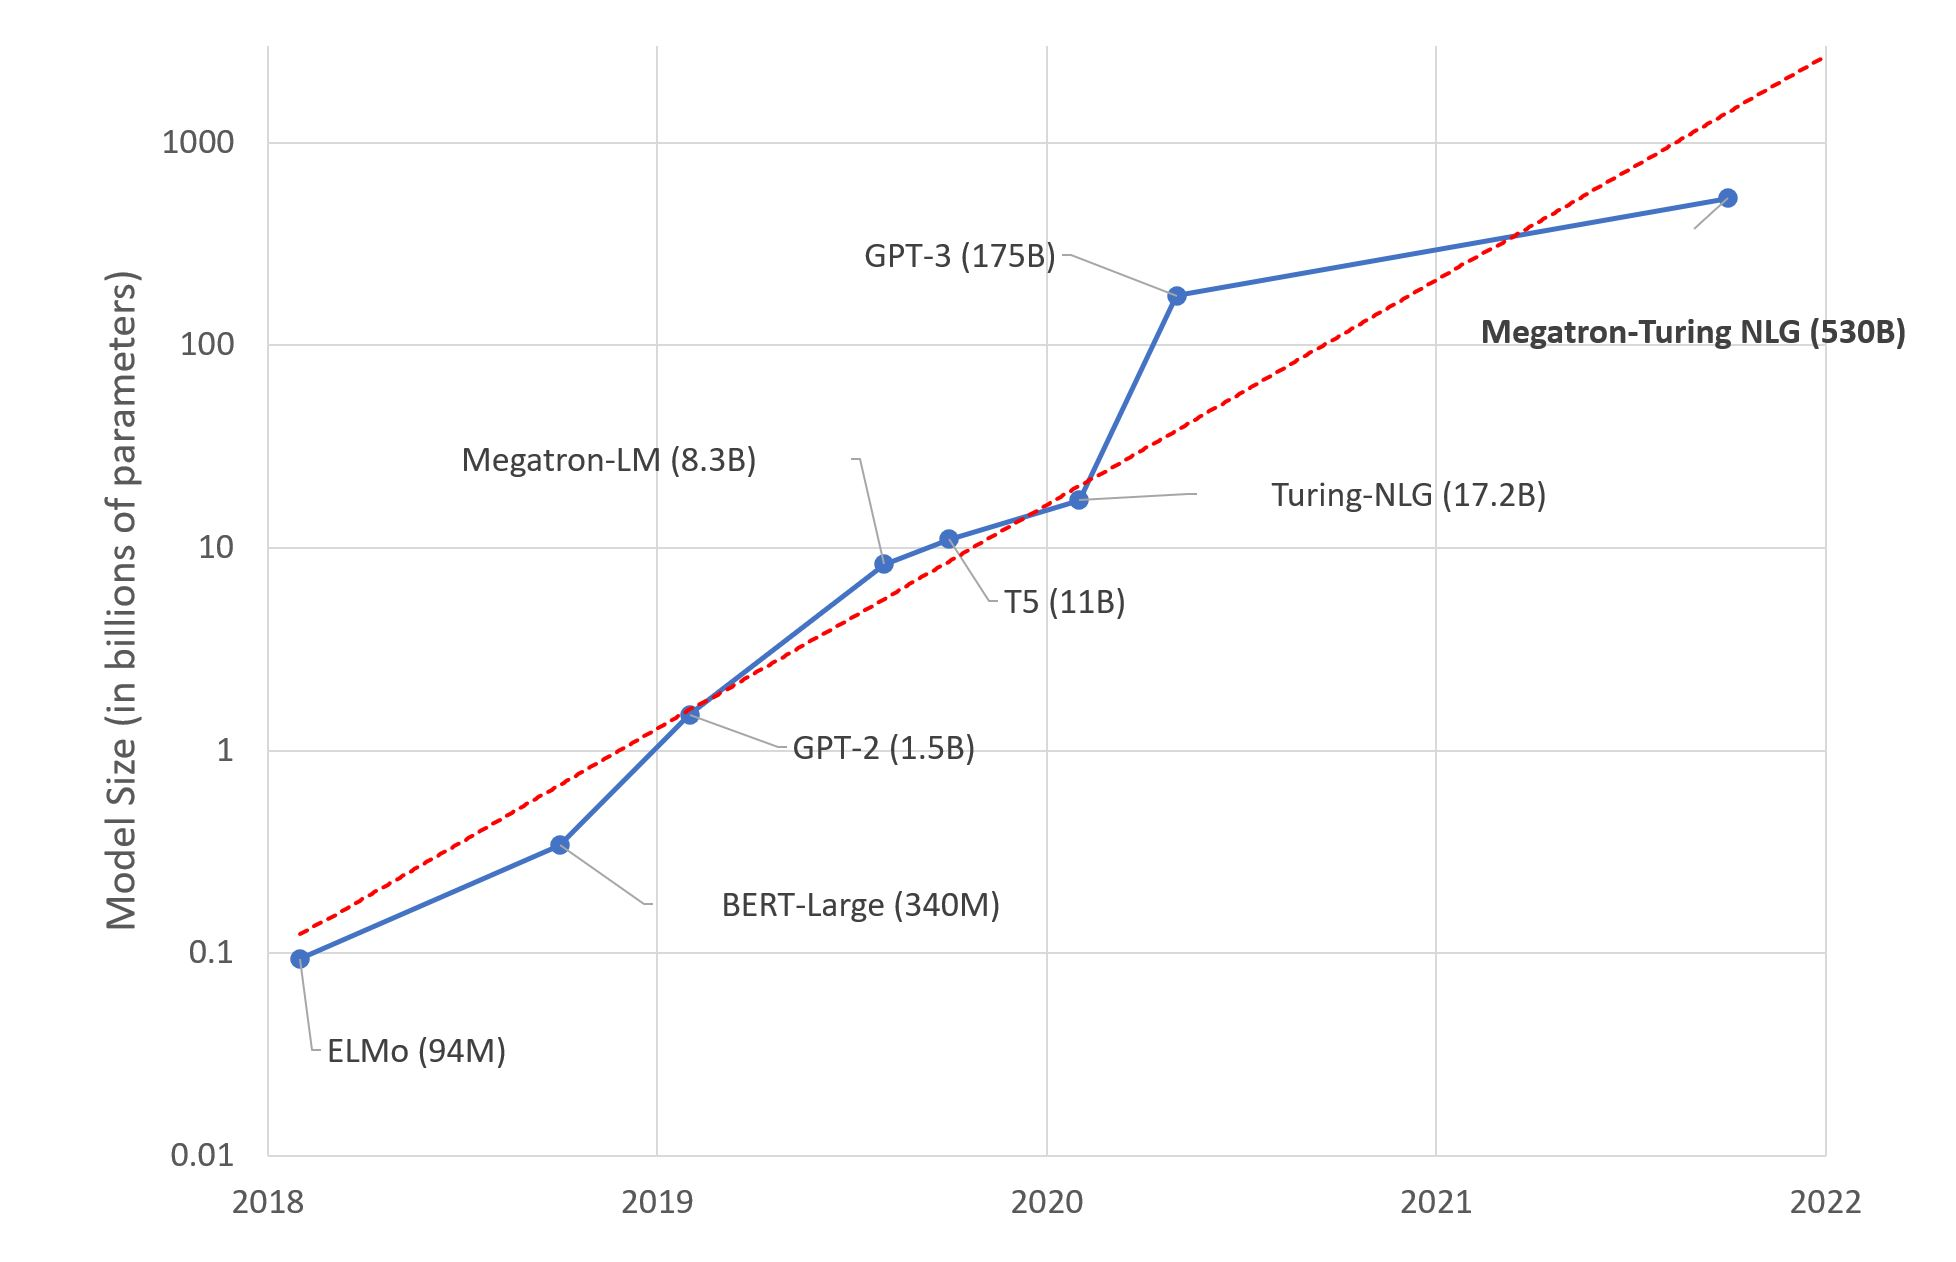
\includegraphics[width=0.65\textwidth]{../images/MegaTron_DeepSpeed_Microsoft_Turing_NLM_model-size-graph.jpg}}

\vspace*{-1cm}

\footnote<.->{\tiny Narayanan et al, 2021}
\end{frame}

\begin{frame}{Large Networks, Large Datasets}
\protect\hypertarget{large-networks-large-datasets-3}{}
\begin{itemize}
\tightlist
\item
  Millions, Billions of network parameters: training demands data
\item
  Most breakthroughs happened on large data; datasets for model training
  get larger and larger

  \begin{itemize}
  \tightlist
  \item
    Vision, Supervised, Self-Supervised: ImageNet-1k (1.4 M images);
    ImageNet-21k (14 M images, \(\approx\) 1.4 TB compressed);
    JFT-300M/4B (300M/4B images); YouTube-8M (8 Million videos, 300 TB)
  \item
    Language-Vision, Self-Supervised

    \begin{itemize}
    \tightlist
    \item
      CLIP trained on WIT-400M (400M image-text pairs); openCLIP on
      LAION-400M/5B (open data, 400M/5B image-text pairs, 11TB/240TB)
    \item
      Stable Diffusion trained on LAION-5B
    \end{itemize}
  \item
    Language, Self-supervised

    \begin{itemize}
    \tightlist
    \item
      GPT-3 trained on 300-400 Billion word tokens
    \item
      LLaMA, RedPajama (open) : 5 TB uncompressed text, ca. 1.2 trillion
      tokens
    \end{itemize}
  \end{itemize}
\end{itemize}

\center{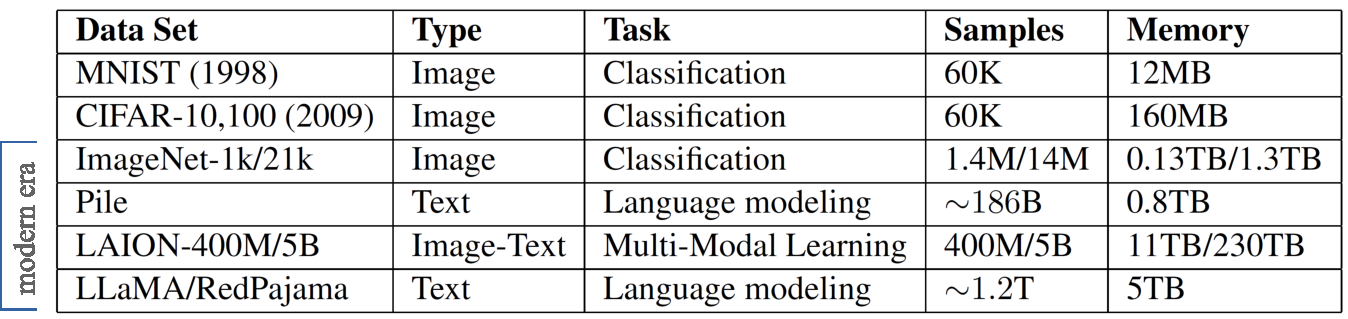
\includegraphics[width=0.8\textwidth]{../images/Datasets_Table_Overview_Small_Large_mod.pdf}}
\end{frame}

\begin{frame}{Reconciling Large Models and Generalization}
\protect\hypertarget{reconciling-large-models-and-generalization}{}
\begin{itemize}
\tightlist
\item
  Both network models and datasets get larger and will continue to grow

  \begin{itemize}
  \tightlist
  \item
    Generalization: large models and the generalization gap
  \end{itemize}
\end{itemize}

\center{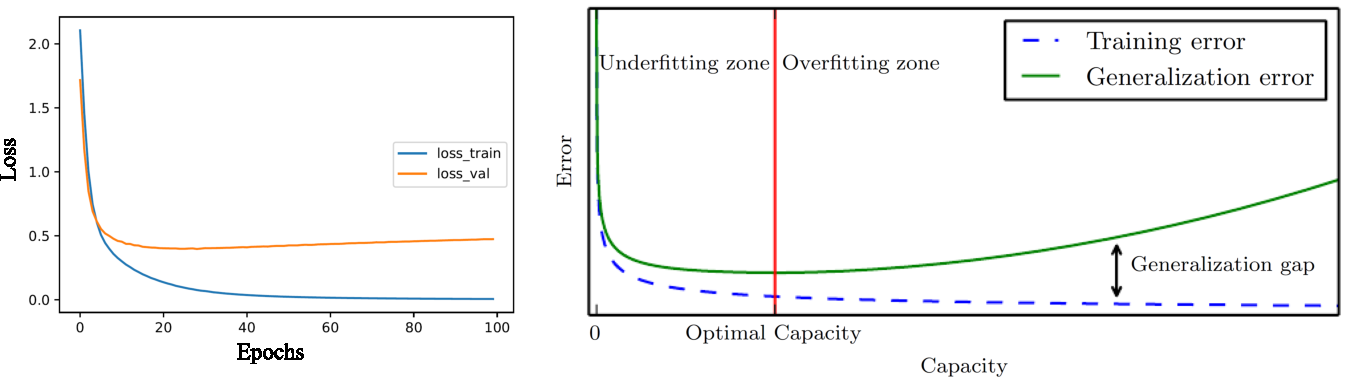
\includegraphics[width=\textwidth]{../images/Generalization_Training_test_Error.pdf}}

\footnote<.->{\tiny Goodfellow et al, 2016}
\end{frame}

\begin{frame}{Reconciling Large Models and Generalization}
\protect\hypertarget{reconciling-large-models-and-generalization-1}{}
\begin{itemize}
\tightlist
\item
  A (classical) simple view - more data, better generalization
\end{itemize}

\center{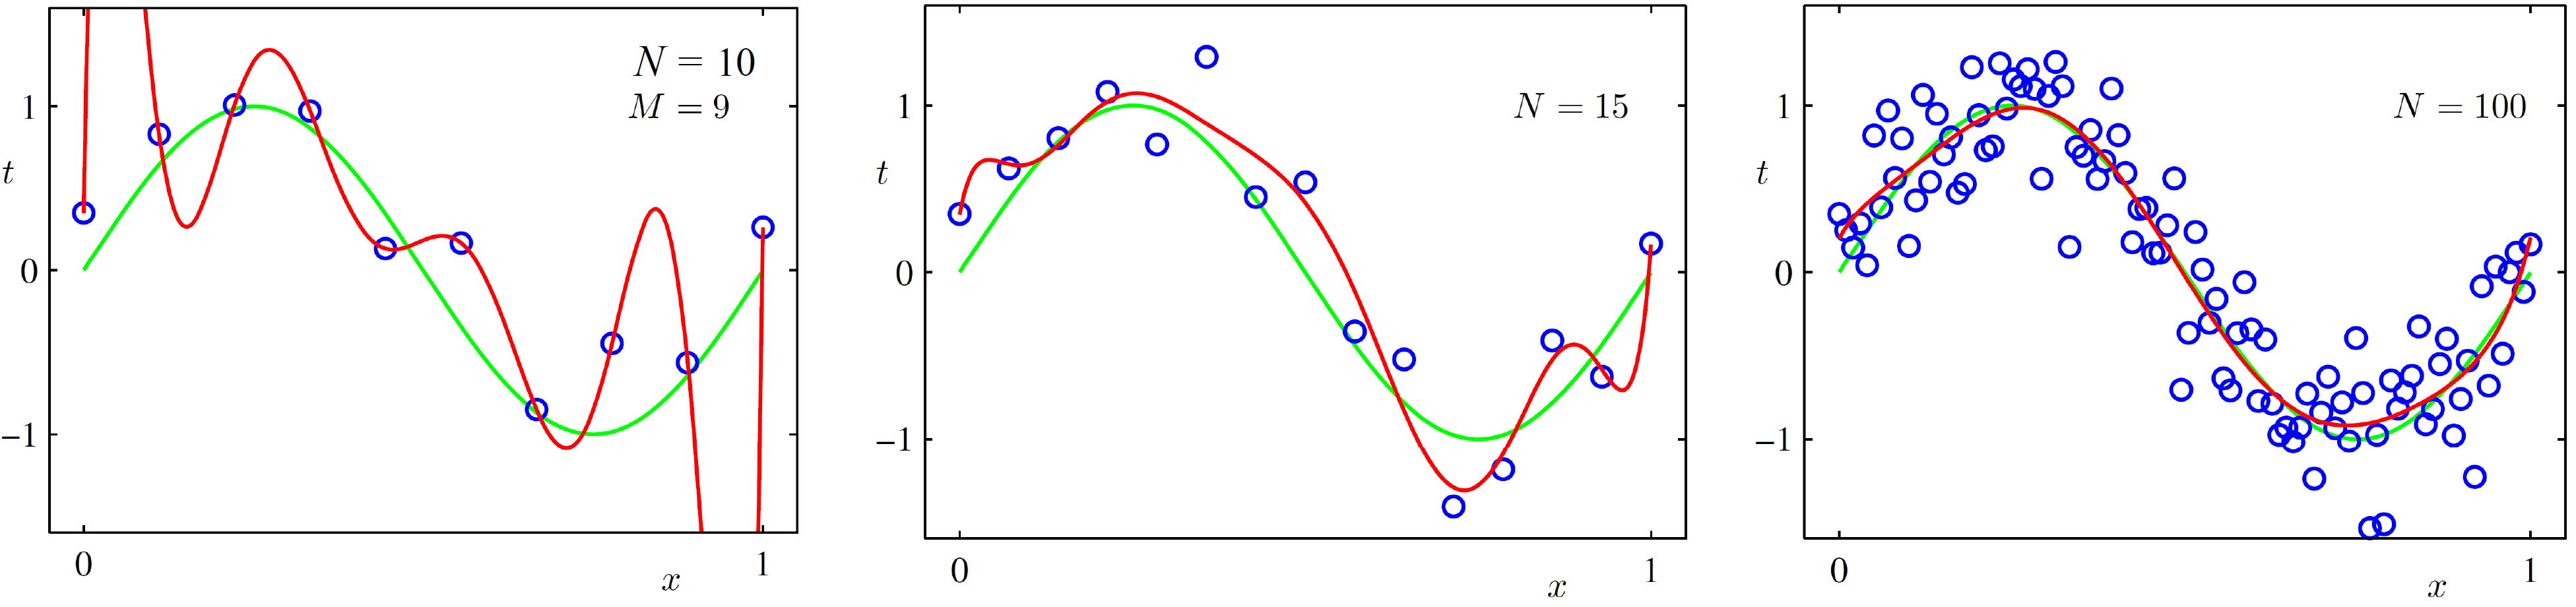
\includegraphics[width=\textwidth]{../images/Simple_Story_More_Data_Toy_Bishop.png}}

\footnote<.->{\tiny Bishop, 2006}
\end{frame}

\begin{frame}{Reconciling Large Models and Generalization}
\protect\hypertarget{reconciling-large-models-and-generalization-2}{}
\begin{itemize}
\tightlist
\item
  A (classical) simple view - more data, better generalization

  \begin{itemize}
  \tightlist
  \item
    Never enough data in higher dimensions - curse of dimensionality
  \end{itemize}
\end{itemize}

\center{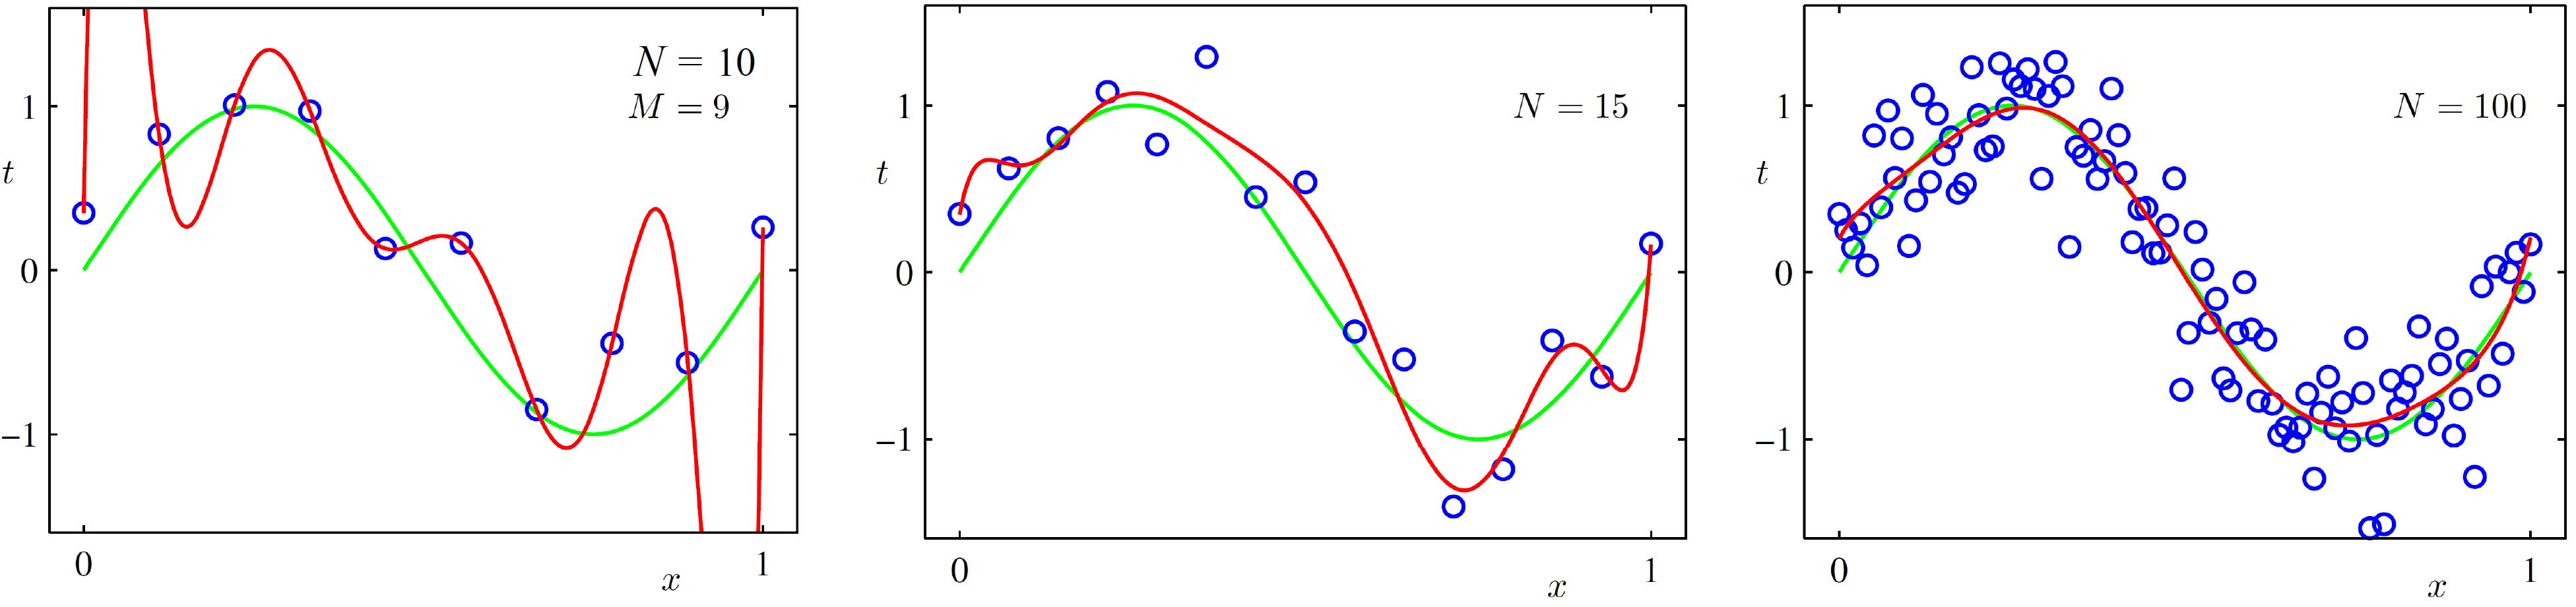
\includegraphics[width=\textwidth]{../images/Simple_Story_More_Data_Toy_Bishop.png}}

\footnote<.->{\tiny Bishop, 2006}
\end{frame}

\begin{frame}{Reconciling Large Models and Generalization}
\protect\hypertarget{reconciling-large-models-and-generalization-3}{}
\begin{itemize}
\tightlist
\item
  A (very recent) complex view - larger models, better generalization

  \begin{itemize}
  \tightlist
  \item
    \textbf{Double descent} test error curve, going beyond
    \textbf{interpolation threshold}
  \item
    Greatly increasing number of model parameters \textbf{reduces}
    generalization gap
  \end{itemize}
\end{itemize}

\center{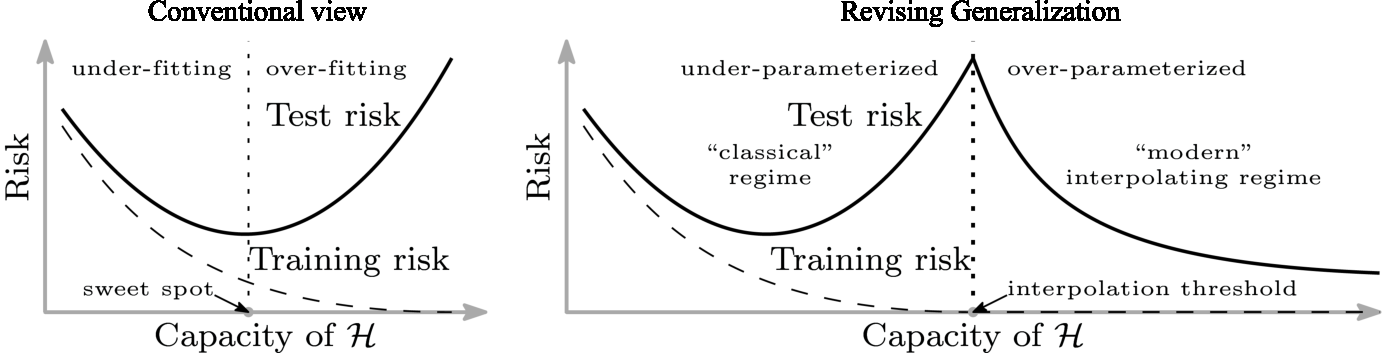
\includegraphics[width=\textwidth]{../images/Conventional_Reconciled_Generalization_View_Belkin_PNAS.pdf}}

\footnote<.->{\tiny Belkin et al, PNAS, 2019}
\end{frame}

\begin{frame}{Reconciling Generalization Gap}
\protect\hypertarget{reconciling-generalization-gap}{}
\center{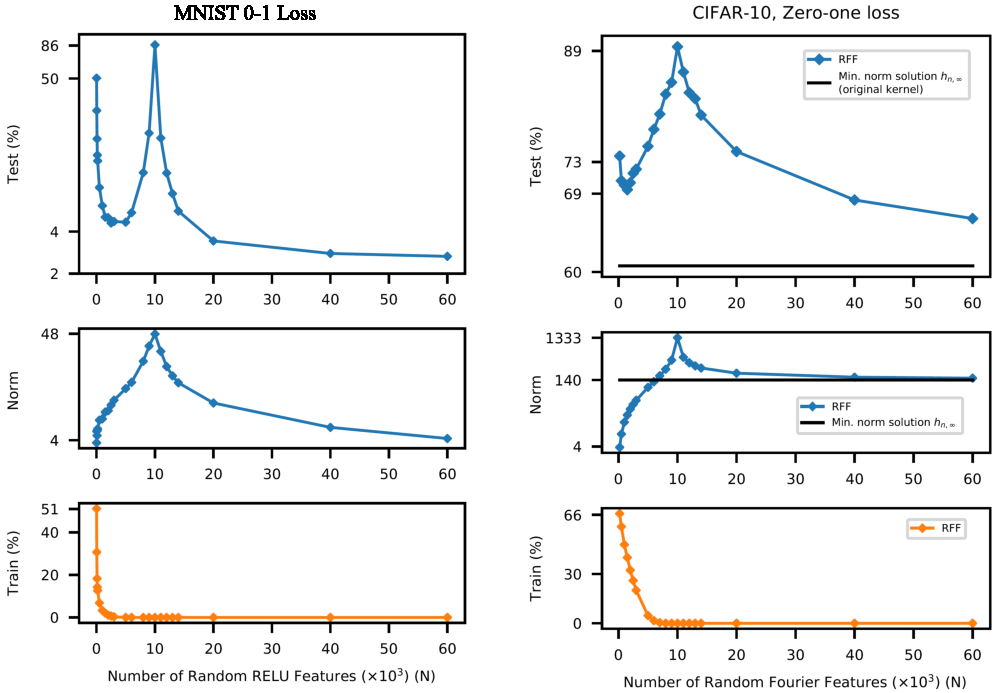
\includegraphics[width=0.8\textwidth]{../images/MNIST_CIFAR_Generalization_Reconciling_Belkin_Test.pdf}}

\footnote<.->{\tiny Belkin et al, PNAS, 2019}
\end{frame}

\begin{frame}{Reconciling Large Models and Generalization}
\protect\hypertarget{reconciling-large-models-and-generalization-4}{}
\begin{itemize}
\tightlist
\item
  Larger models generalize better

  \begin{itemize}
  \tightlist
  \item
    Reconciling generalization - large, overparameterized models
    generalize strongly
  \item
    Greatly increasing number of model parameters \textbf{reduces}
    generalization gap
  \item
    \textbf{Double descent} test error curves
  \end{itemize}
\end{itemize}

\center{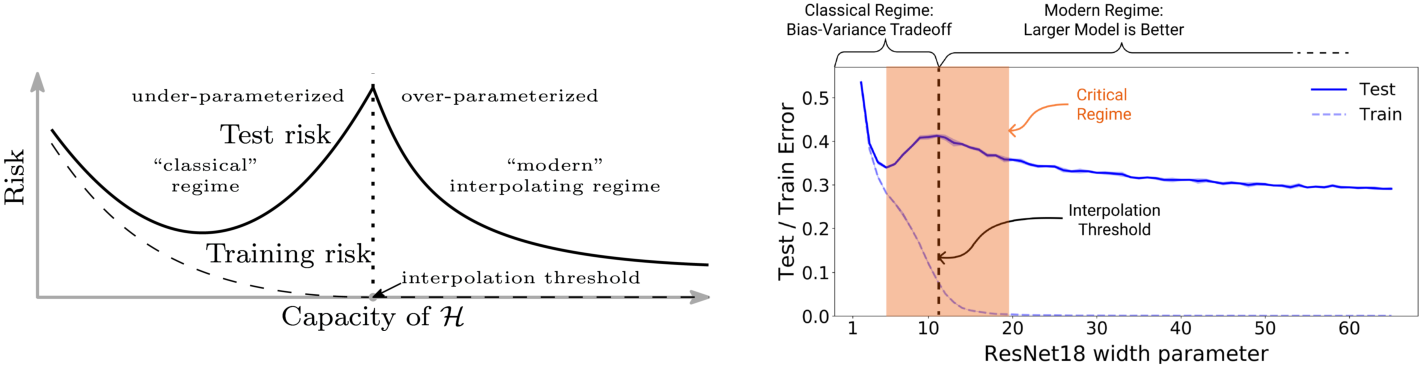
\includegraphics[width=\textwidth]{../images/Double_Descent_Large_Models_mod.pdf}}

\footnote<.->{\tiny Belkin et al, PNAS, 2019, Nakkiran et al, ICLR, 2020}
\end{frame}

\begin{frame}{Large Models and Generalization}
\protect\hypertarget{large-models-and-generalization}{}
\begin{itemize}
\tightlist
\item
  Larger models generalize better

  \begin{itemize}
  \tightlist
  \item
    Evidence across different large scale training scenarios
  \end{itemize}
\end{itemize}

\center{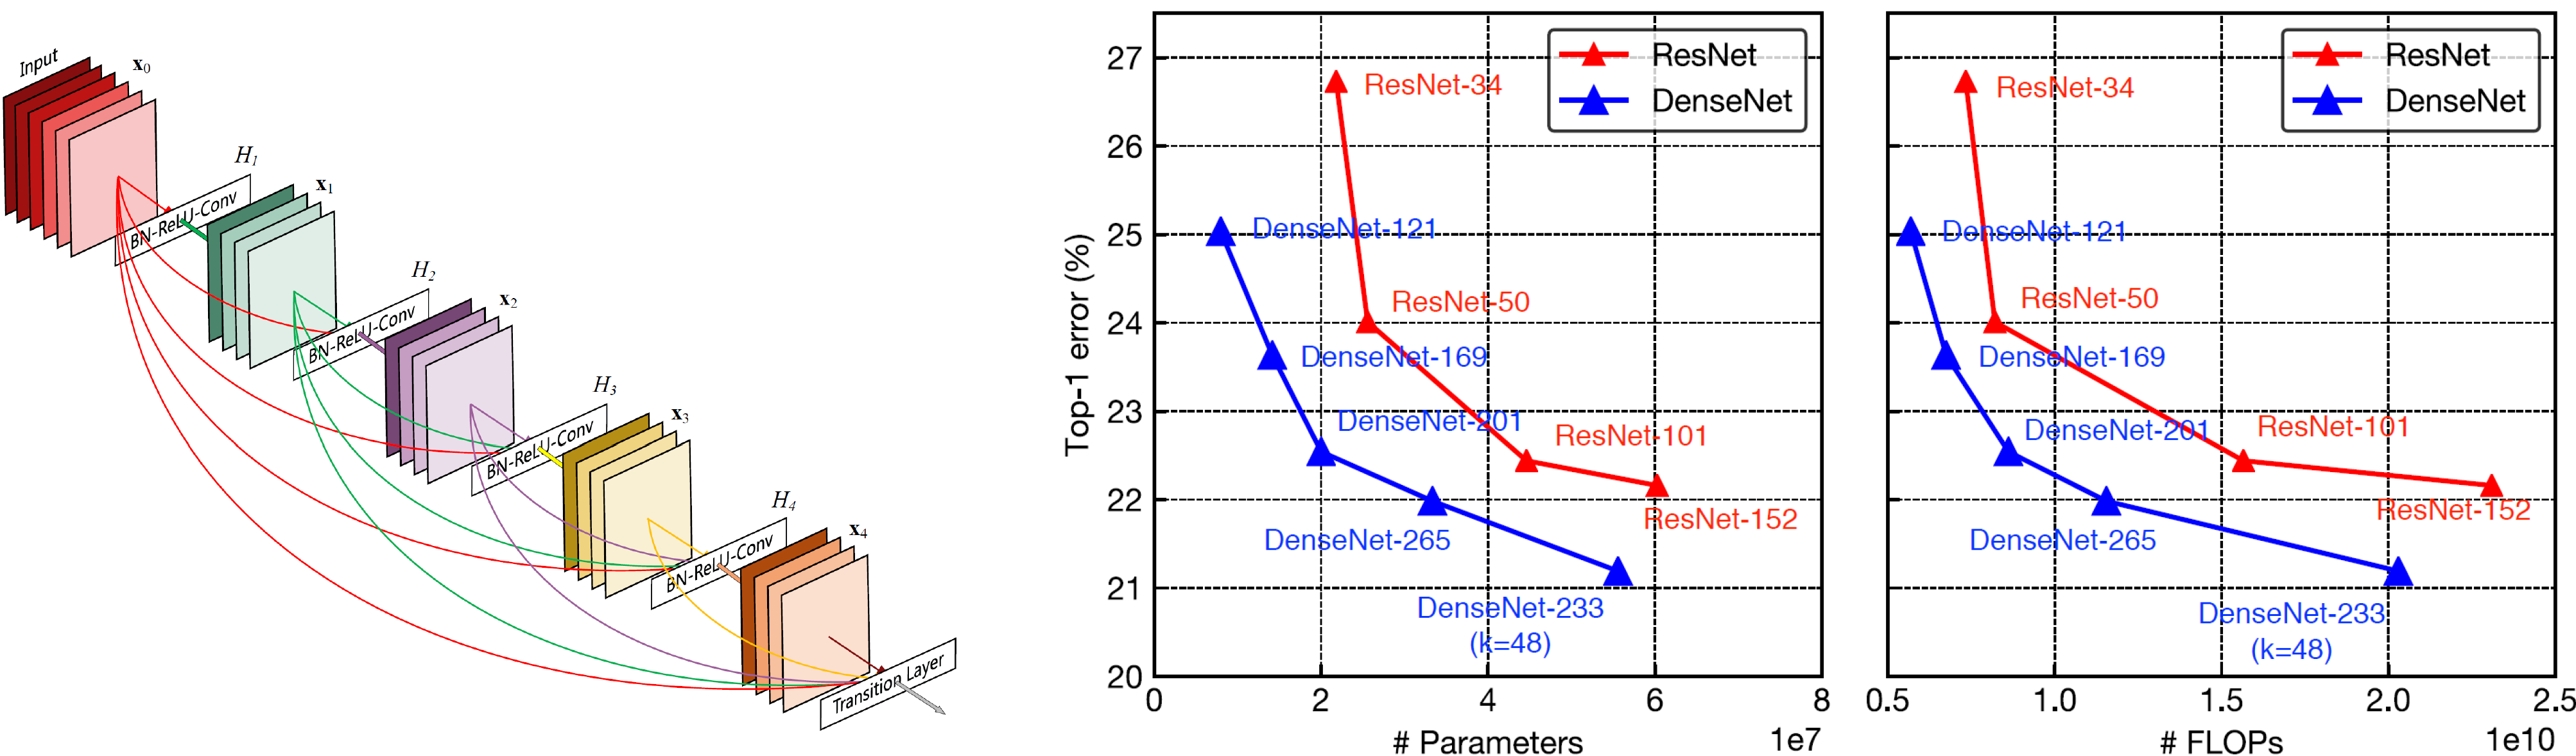
\includegraphics[width=\textwidth]{../images/ResNet_DenseNet_Improving_Model_Size_ImageNet-1k.png}}

\footnote<.->{\tiny Huang et al, CVPR, 2017}
\end{frame}

\begin{frame}{Large Models and Generalization}
\protect\hypertarget{large-models-and-generalization-1}{}
\begin{itemize}
\tightlist
\item
  Larger models generalize better

  \begin{itemize}
  \tightlist
  \item
    Evidence across different large scale training scenarios
  \end{itemize}
\end{itemize}

\center{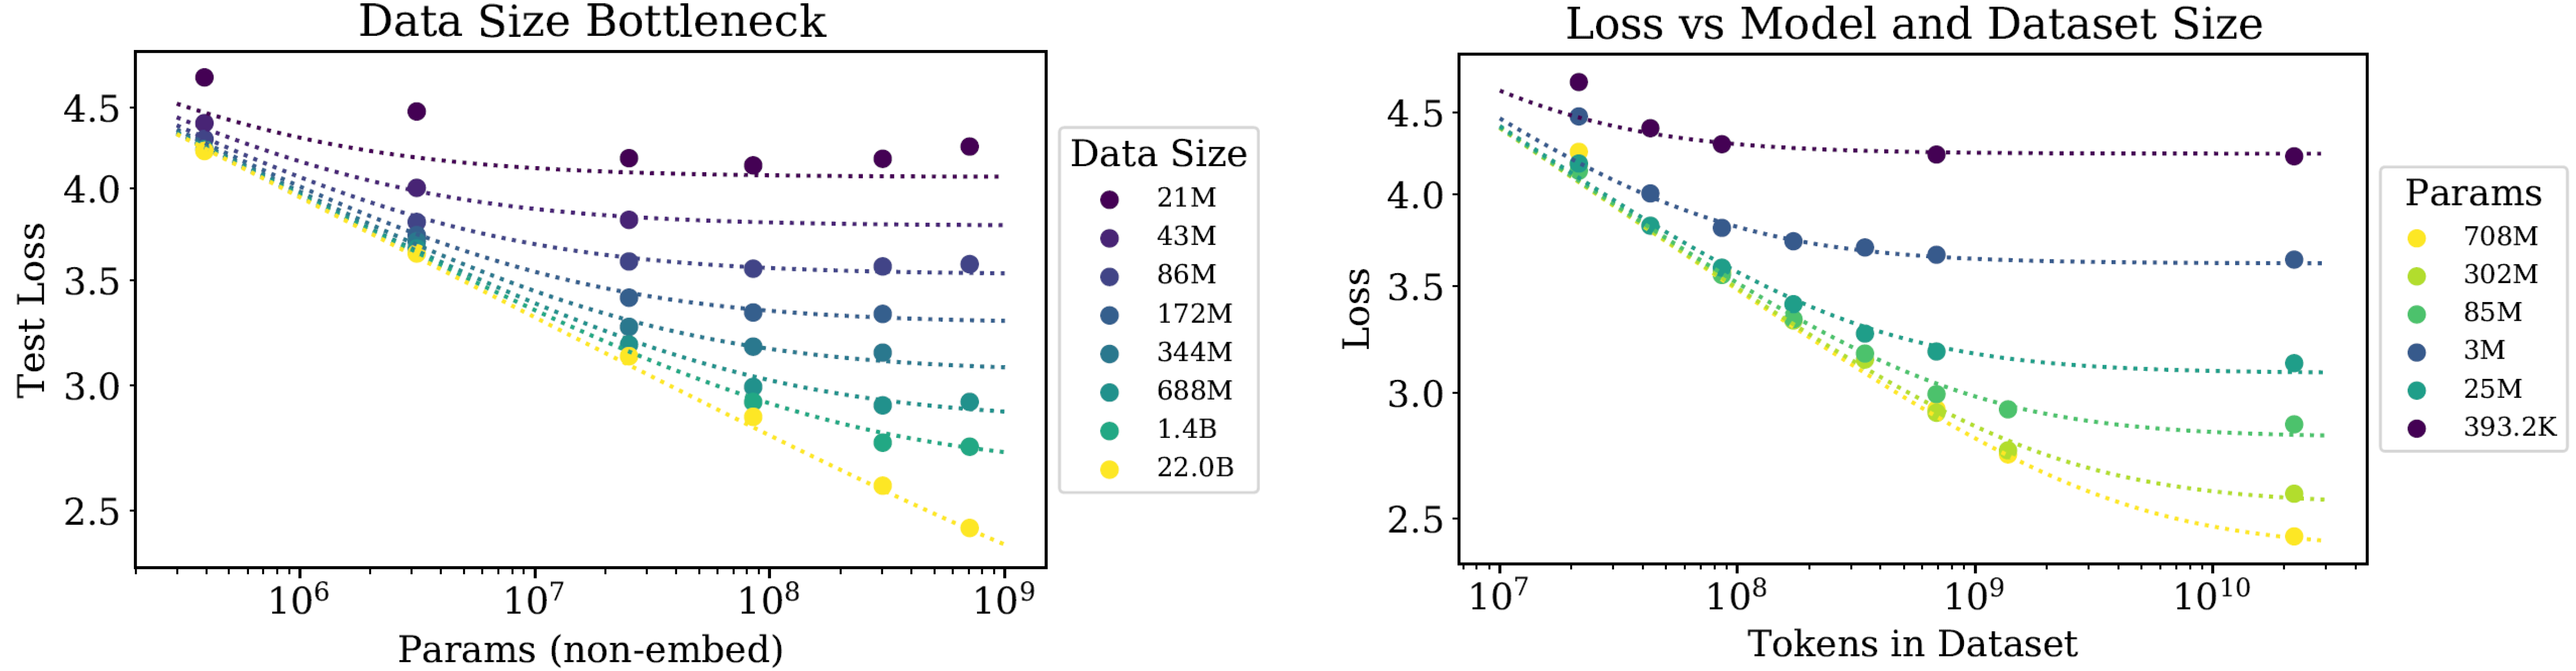
\includegraphics[width=\textwidth]{../images/GPT_Model_and_Data_size_Test_error.png}}

\footnote<.->{\tiny Kaplan et al, 2020; Brown et al, NeurIPS, 2020}
\end{frame}

\begin{frame}{Large Models and Large Data}
\protect\hypertarget{large-models-and-large-data}{}
\begin{itemize}
\tightlist
\item
  Scaling Laws: given sufficient compute budget, increasing both model
  size and data size is the way to further strongly boost generalization
\end{itemize}

\center{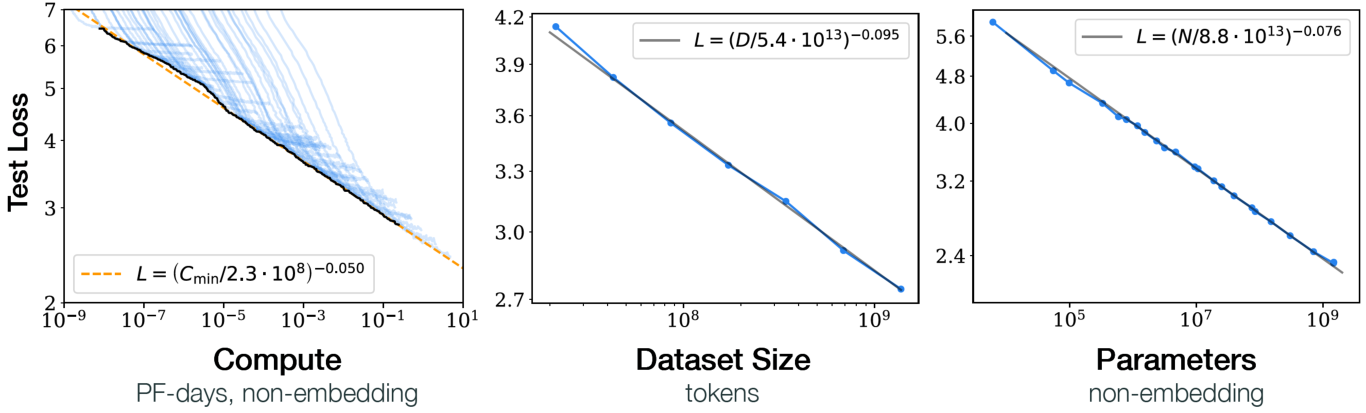
\includegraphics[width=\textwidth]{../images/Scaling_Compute_Data_Model_Size_Performance_Increase_Kaplan_Test.pdf}}

\footnote<.->{\tiny Kaplan et al, 2020}
\end{frame}

\begin{frame}{Large Models and Large Data}
\protect\hypertarget{large-models-and-large-data-1}{}
\begin{itemize}
\tightlist
\item
  Increasing model size is \textbf{good} idea, provided enough compute
  and data
\end{itemize}

\center{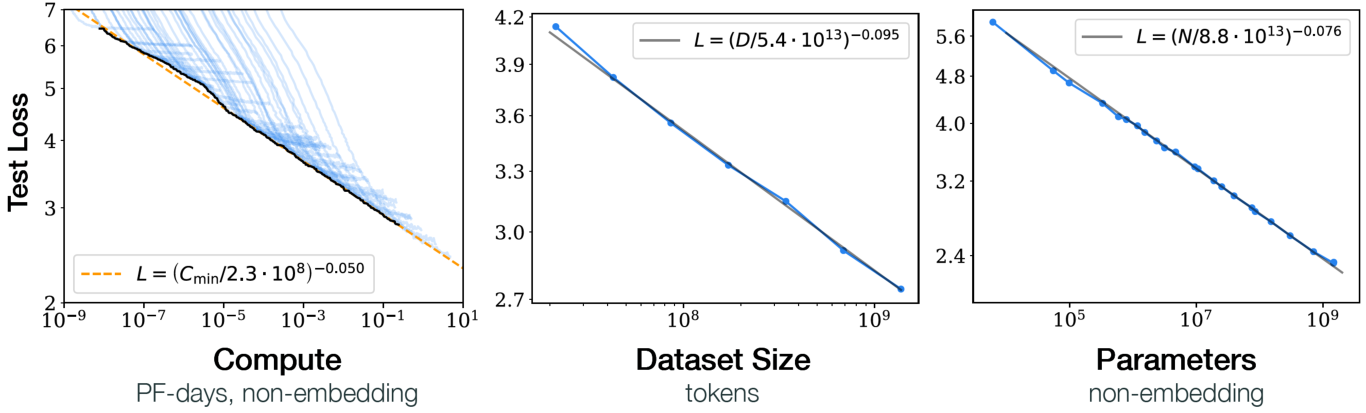
\includegraphics[width=\textwidth]{../images/Scaling_Compute_Data_Model_Size_Performance_Increase_Kaplan_Test.pdf}}

\footnote<.->{\tiny Kaplan et al, 2020}
\end{frame}

\begin{frame}{Large Models, Data and Generalization}
\protect\hypertarget{large-models-data-and-generalization}{}
\begin{itemize}
\tightlist
\item
  Language Modeling : very large models, very large data, generic
  self-supervised pre-training (autoregressive generative sequence
  models)

  \begin{itemize}
  \tightlist
  \item
    GPT-3, trained on Common Crawl \& co (300-400B word token samples)
  \item
    Strong few-show and zero-shot transfer at largest scale (175B
    params)
  \end{itemize}
\end{itemize}

\center{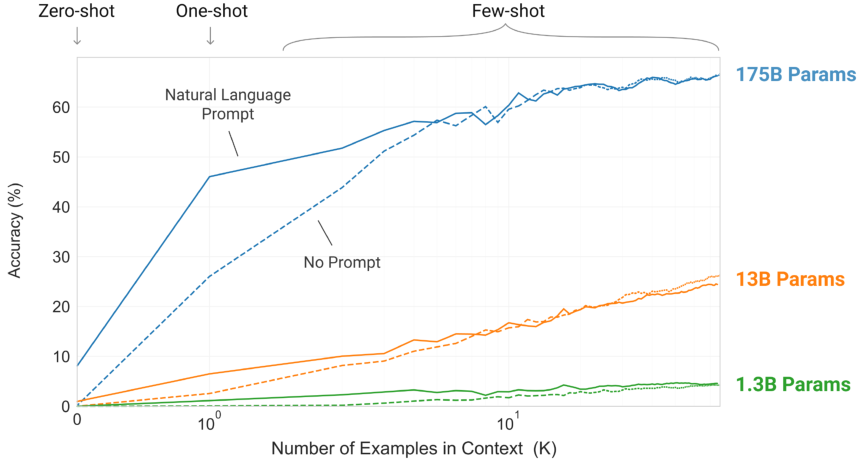
\includegraphics[width=0.7\textwidth]{../images/GPT_Model_size_few_shot_context_performance_mod.pdf}}

\footnote<.->{\tiny Brown et al, NeurIPS, 2020}
\end{frame}

\begin{frame}{Large Models, Data and Generalization}
\protect\hypertarget{large-models-data-and-generalization-1}{}
\begin{itemize}
\tightlist
\item
  Larger models transfer better

  \begin{itemize}
  \tightlist
  \item
    Evidence across different large scale training scenarios
  \item
    Using large models (BiT - Big Transfer, ResNet-152x4: 928M params),
    large data

    \begin{itemize}
    \tightlist
    \item
      ImageNet-21k, \(\sim 14\)M images (instead of standard
      ImageNet-1k, \(\sim 1.4\)M)
    \item
      JFT-300M : \(\approx\) 18K classes, noisy labels, 300x larger than
      ImageNet-1k
    \end{itemize}
  \item
    Pre-training a single large model: \textbf{81 hours} with
    \textbf{256 A100} GPUs (20k GPU hours; ImageNet-21k, JUWELS Booster)
  \end{itemize}
\end{itemize}

\center{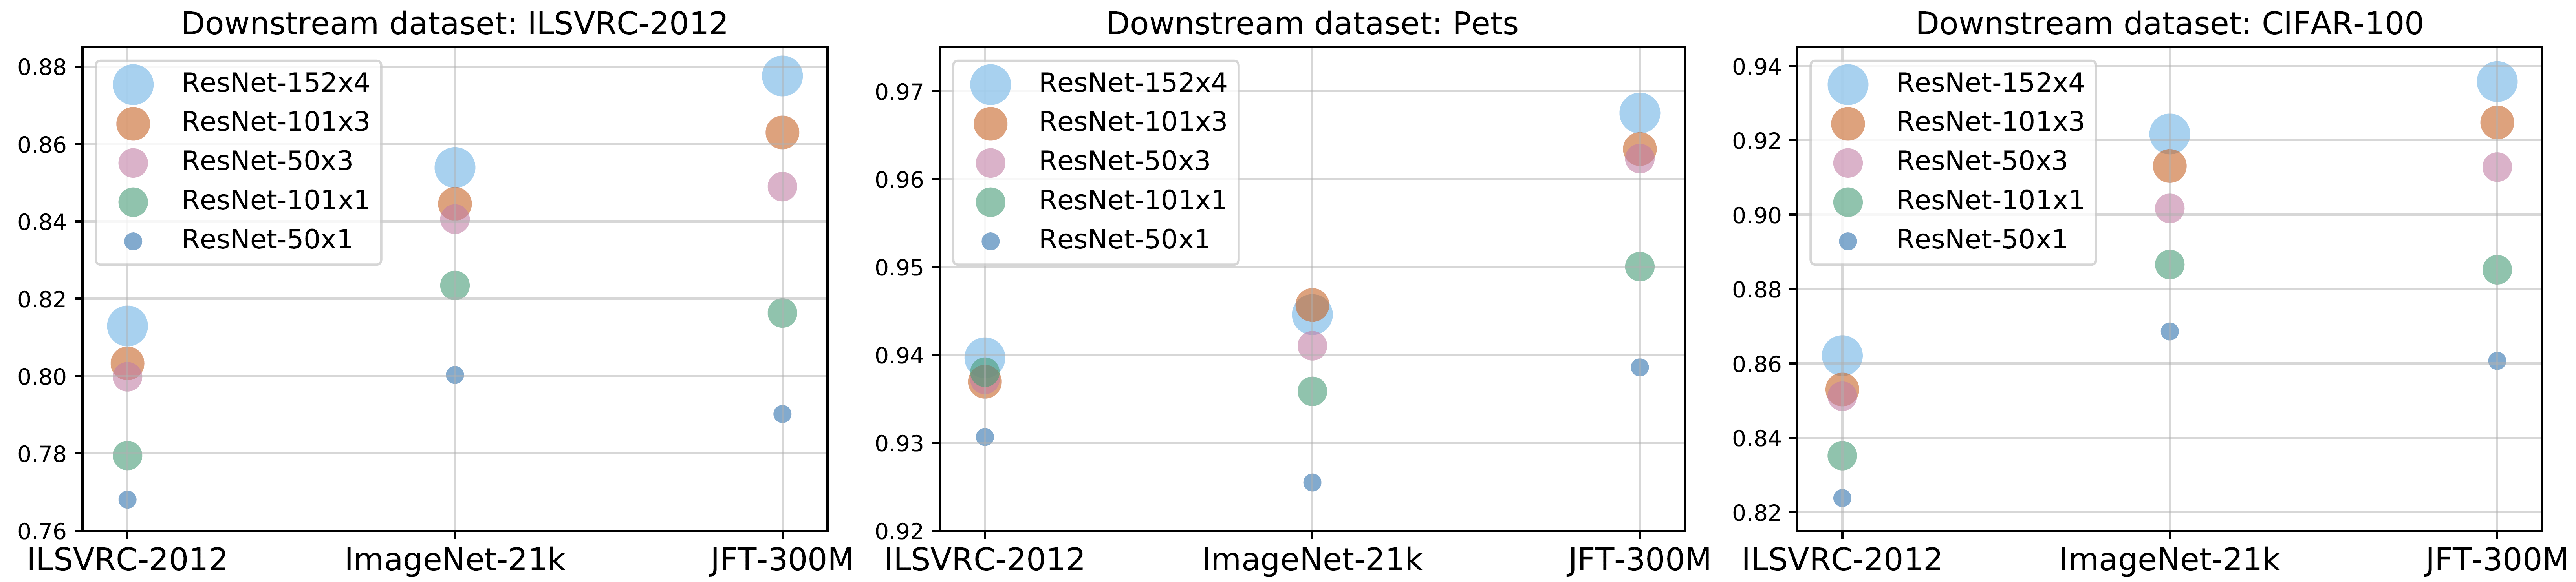
\includegraphics[width=\textwidth]{../images/Pretraining_BiT_Data_Networks_smaller_larger.png}}

\footnote<.->{\tiny BiT - Big Transfer, Kolesnikov et al, ECCV, 2020}
\end{frame}

\begin{frame}{Large Models, Data and Generalization}
\protect\hypertarget{large-models-data-and-generalization-2}{}
\begin{itemize}
\tightlist
\item
  Self-supervised language-vision pre-training: GPT for multi-modal
  image-text data

  \begin{itemize}
  \tightlist
  \item
    CLIP: very strong zero- and few-shot transfer across various targets
  \item
    very large data for pre-training (eg. open LAION-400M/5B, image-text
    pairs)
  \end{itemize}
\item
  Larger model and data scale - better zero- and few-shot transfer
\end{itemize}

\center{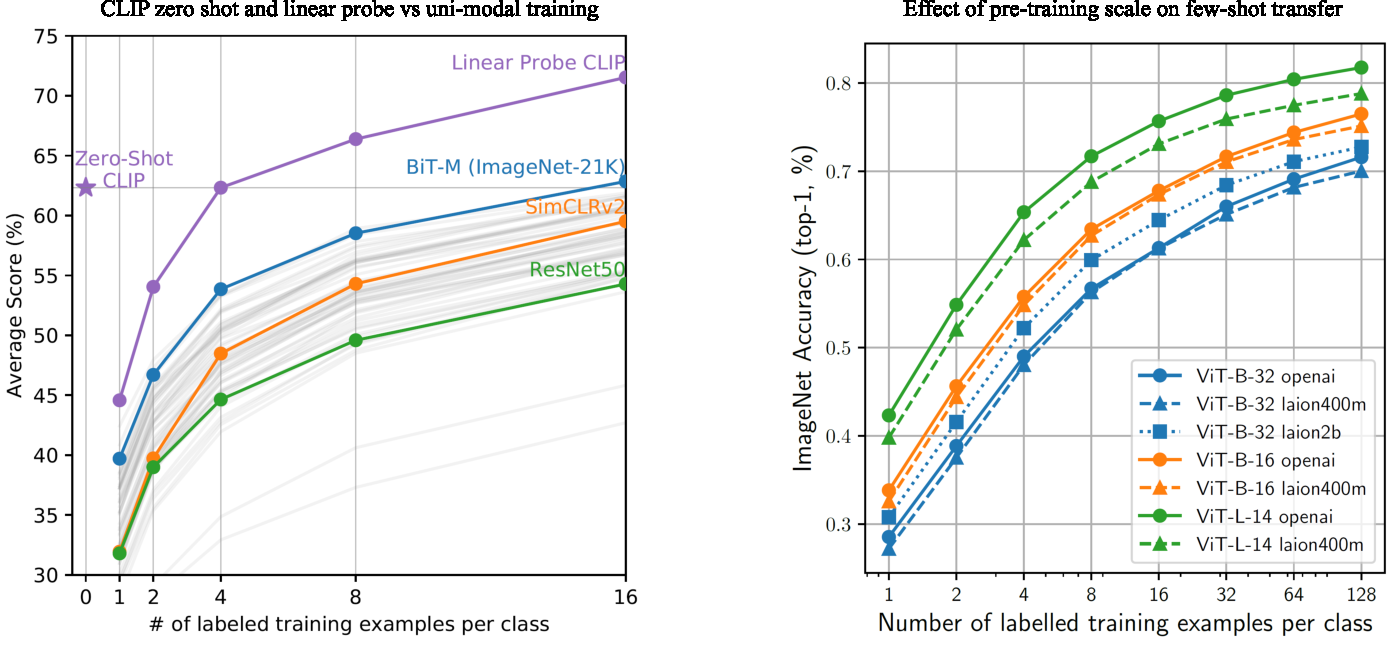
\includegraphics[width=0.85\textwidth]{../images/CLIP_Zero_Shot_Few_Shot_Scaling_mod.pdf}}

\footnote<.->{\tiny Radford, ICML, 2021; Schumann et al, NeurIPS 2022}
\end{frame}

\begin{frame}{Large Models, Data and Generalization}
\protect\hypertarget{large-models-data-and-generalization-3}{}
\begin{itemize}
\tightlist
\item
  Larger model and data scale - better zero-shot transfer

  \begin{itemize}
  \tightlist
  \item
    \textbf{88 hours} with \textbf{400 A100} (50K GPU hours) for
    training of ViT L/14 openCLIP on LAION-400M (JUWELS Booster)
  \end{itemize}
\end{itemize}

\center{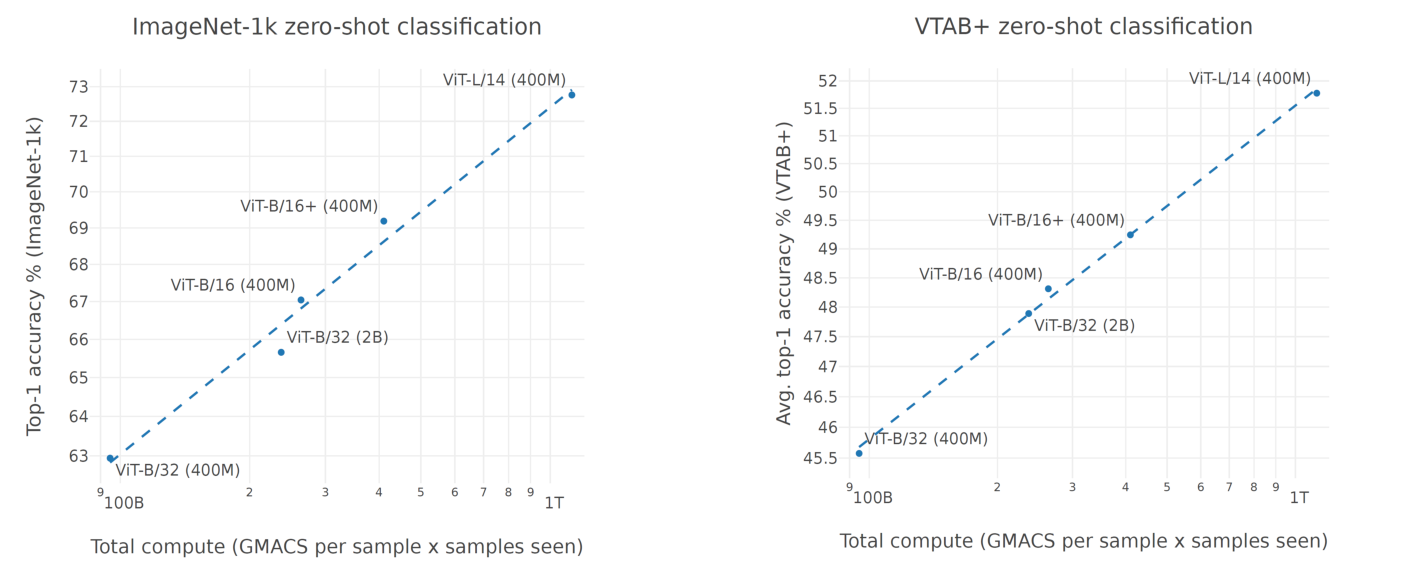
\includegraphics[width=\textwidth]{../images/LAION_openCLIP_scaling_zero_shot_mod.pdf}}

\footnote<.->{\tiny Schumann et al, NeurIPS, 2022}
\end{frame}

\begin{frame}{Large Models, Data and Generalization}
\protect\hypertarget{large-models-data-and-generalization-4}{}
\begin{block}{Summary}
\protect\hypertarget{summary}{}
\begin{itemize}
\tightlist
\item
  Theoretical insights suggest revision of model generalization at
  larger scales

  \begin{itemize}
  \tightlist
  \item
    generalization can improve with larger model scales\\
  \end{itemize}
\item
  Scaling laws suggest that larger scales may be one key to strong
  generalization, model robustness and transferability
\item
  Major breakthroughs in model transferability and robustness in
  language (GPT) and vision (ViT, CLIP) when using very large model,
  data and compute scale
\item
  Experiments involving strongly transferable models at larger scale are
  extremely compute intensive

  \begin{itemize}
  \tightlist
  \item
    ten or hundred thousands of GPU hours
  \end{itemize}
\end{itemize}
\end{block}
\end{frame}

\begin{frame}{Distributed Training with Large Data}
\protect\hypertarget{distributed-training-with-large-data}{}
\begin{itemize}
\tightlist
\item
  ImageNet: transition to modern deep learning era;

  \begin{itemize}
  \tightlist
  \item
    outstanding effort in large data collection (Fei-Fei et al,
    Stanford)
  \item
    building dataset via crowdsourcing over 4 years
  \end{itemize}
\end{itemize}

\center{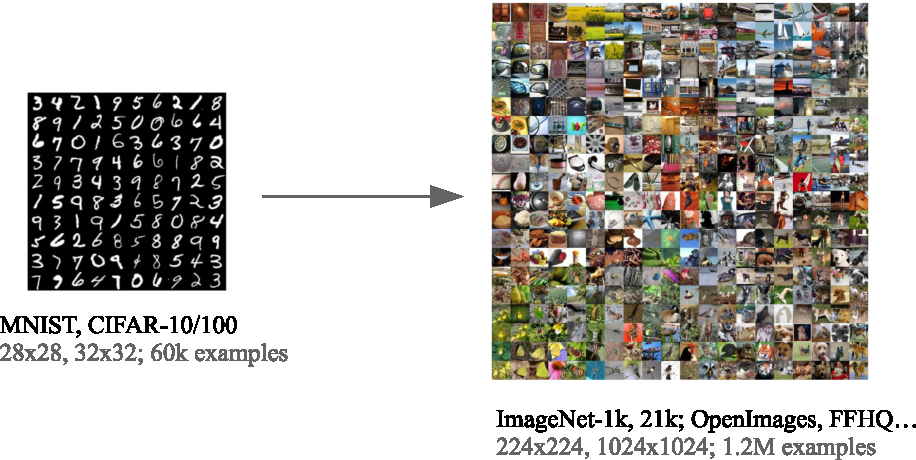
\includegraphics[width=0.8\textwidth]{../images/MNIST_CIFAR_ImageNet_Transition_Test.pdf}}
\end{frame}

\begin{frame}{Distributed Training on ImageNet}
\protect\hypertarget{distributed-training-on-imagenet}{}
\begin{itemize}
\tightlist
\item
  Full dataset (ImageNet-21k) : 14M images, 21k classes labeled
\item
  ImageNet-1k : dataset for ILSVRC competition (2010 - 2017), 1k classes

  \begin{itemize}
  \tightlist
  \item
    1.28M Training, 100k Test, 50k Validation sets
  \item
    usual image resolution used for training: 224x224
  \item
    current accuracies : \(> 88\%\) top-1, \(>97\%\) top-5
  \end{itemize}
\end{itemize}

\center{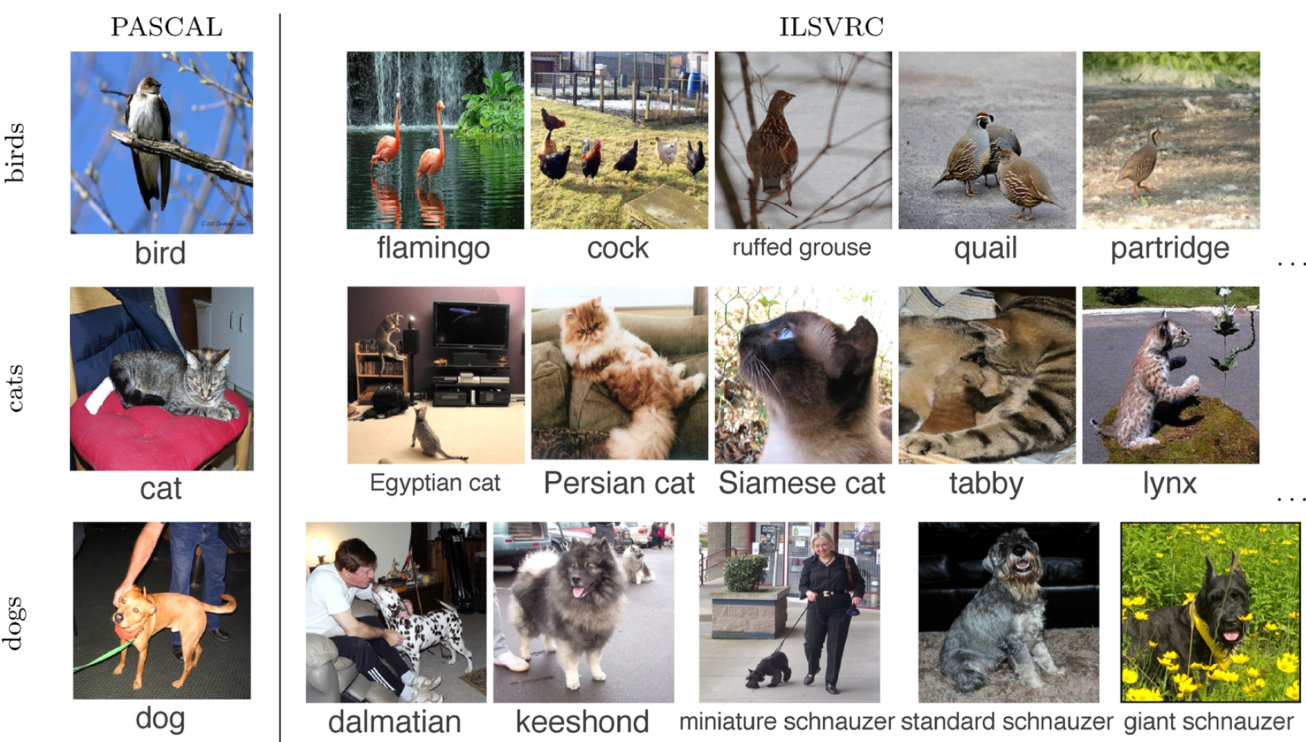
\includegraphics[width=0.6\textwidth]{../images/ImageNet_Pascal_Transition_Test.pdf}}

\footnote<.->{\tiny Russakovsky et al, IJCV, 2015}
\end{frame}

\begin{frame}{Distributed Training on ImageNet}
\protect\hypertarget{distributed-training-on-imagenet-1}{}
\begin{itemize}
\tightlist
\item
  Full dataset (ImageNet-21k) : 14M images, 21k classes labeled
\item
  ImageNet-1k : dataset for ILSVRC competition (2010 - 2017), 1k classes

  \begin{itemize}
  \tightlist
  \item
    1.28M Training, 100k Test, 50k Validation sets
  \item
    usual image resolution used for training: 224x224
  \item
    current accuracies : \(> 88\%\) top-1, \(>97\%\) top-5
  \end{itemize}
\end{itemize}

\center{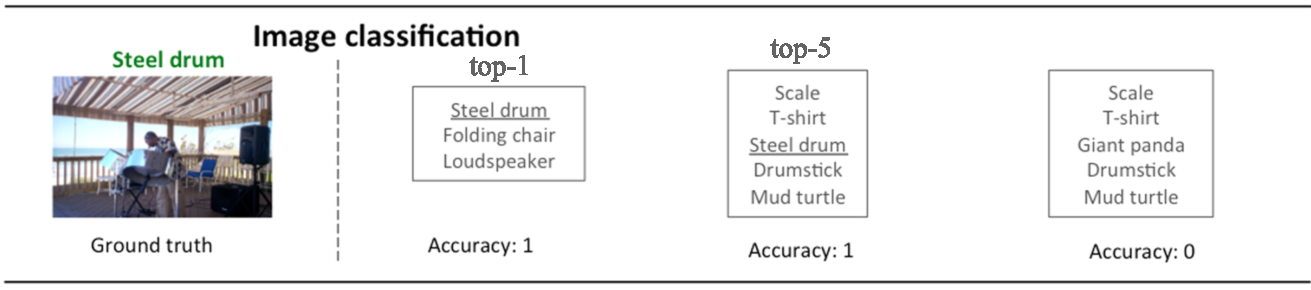
\includegraphics[width=0.8\textwidth]{../images/ImageNet_Accuracy_Detection_Top_Only_Test.pdf}}

\footnote<.->{\tiny Russakovsky et al, IJCV, 2015}
\end{frame}

\begin{frame}{Distributed Training on ImageNet}
\protect\hypertarget{distributed-training-on-imagenet-2}{}
\begin{itemize}
\tightlist
\item
  ImageNet-1k : still gold standard in training large visual recognition
  models

  \begin{itemize}
  \tightlist
  \item
    pre-trained models: transfer learning on more specific smaller
    datasets
  \end{itemize}
\item
  ResNet-50 : baseline model network, accuracies : \(\approx 75\%\)
  top-1, \(\approx 94\%\) top-5 (Winner ILSVRC 2015)
\end{itemize}

\center{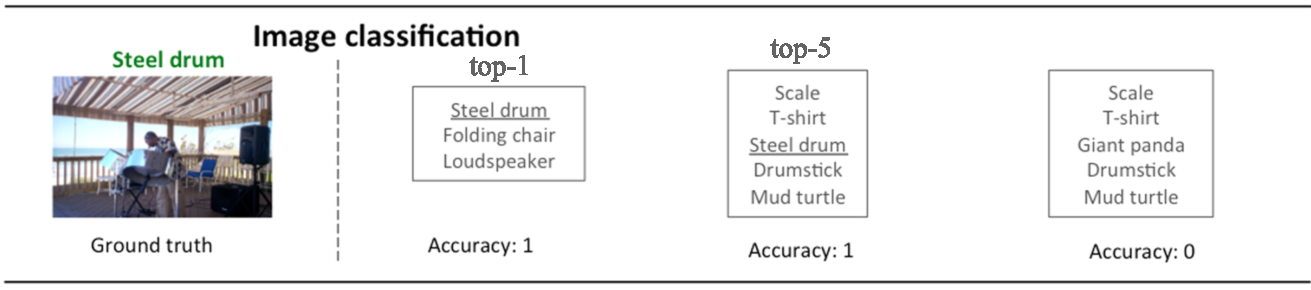
\includegraphics[width=0.8\textwidth]{../images/ImageNet_Accuracy_Detection_Top_Only_Test.pdf}}

\footnote<.->{\tiny Russakovsky et al, IJCV, 2015}
\end{frame}

\begin{frame}{Distributed Training on ImageNet}
\protect\hypertarget{distributed-training-on-imagenet-3}{}
\begin{itemize}
\tightlist
\item
  ResNet-50 : efficient distributed training in data parallel mode
  possible

  \begin{itemize}
  \tightlist
  \item
    25M weights, 103Mb for activations, model training on 224x224
    ImageNet-1k
  \item
    \(\approx 4\) GB Memory with \(B_{ref}=64\) : fits onto single GPU
  \end{itemize}
\end{itemize}

\center{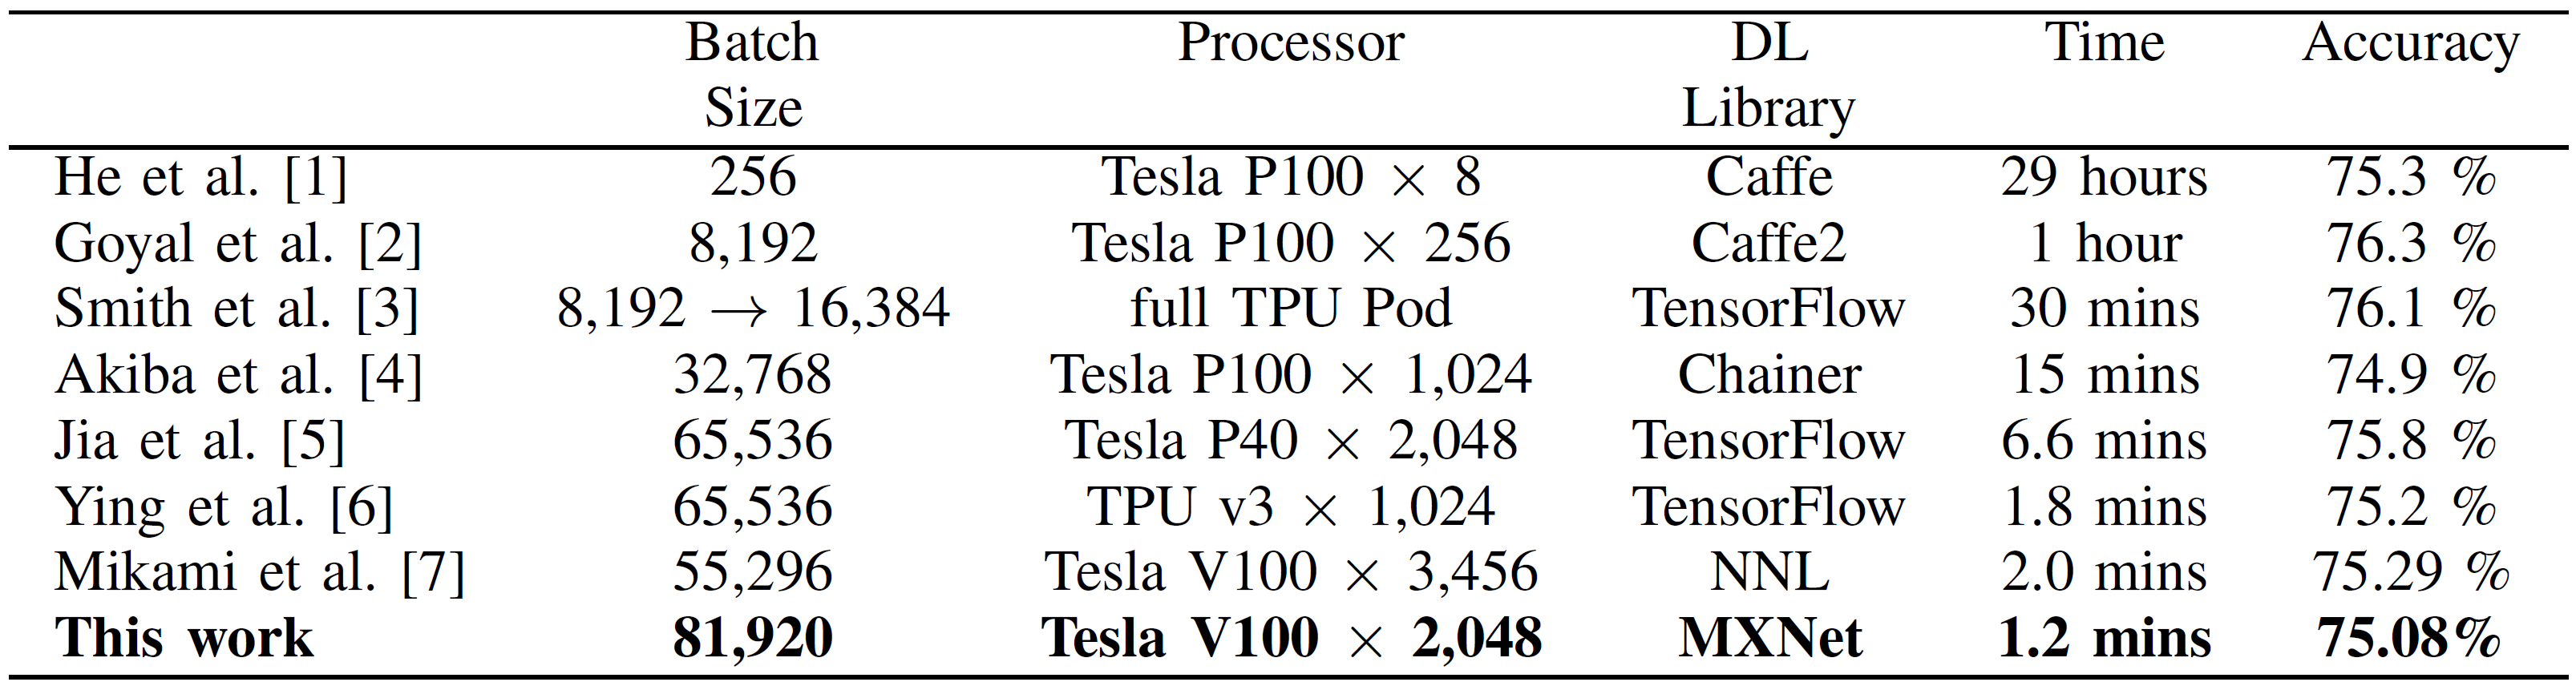
\includegraphics[width=0.6\textwidth]{../images/Yamazaki_RunTime_Table_ImageNet_ResNet-50_Accuracies.png}}

\center{ \hspace*{5cm} 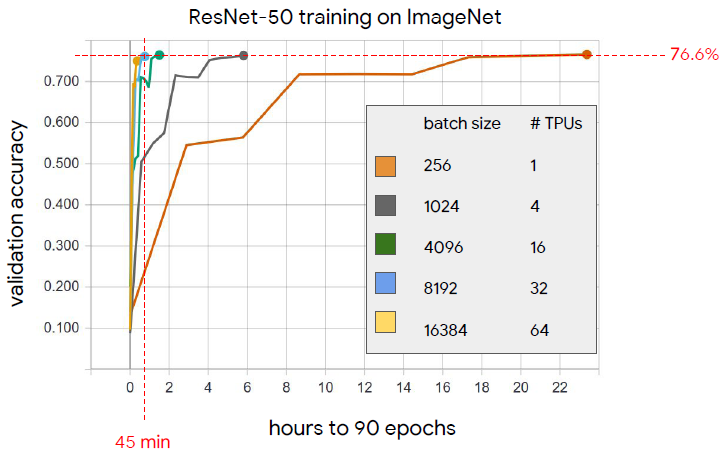
\includegraphics[width=0.4\textwidth]{../images/ResNet-50_ImageNet_Training_Time_Validation_Accuracy.png}}

\vspace*{-1cm}

\footnote<.->{\tiny Yamazoto et al, 2019; Ying, 2018}
\end{frame}

\begin{frame}{Distributed Training on ImageNet}
\protect\hypertarget{distributed-training-on-imagenet-4}{}
\begin{itemize}
\tightlist
\item
  Efficient distributed training in data parallel mode

  \begin{itemize}
  \tightlist
  \item
    requires good scaling of throughput Images/sec during training
  \item
    image throughput during training ideally increasing as
    \(\tau_K^{*} = K \cdot \tau_{ref}\) Images/sec
  \end{itemize}
\end{itemize}

\center{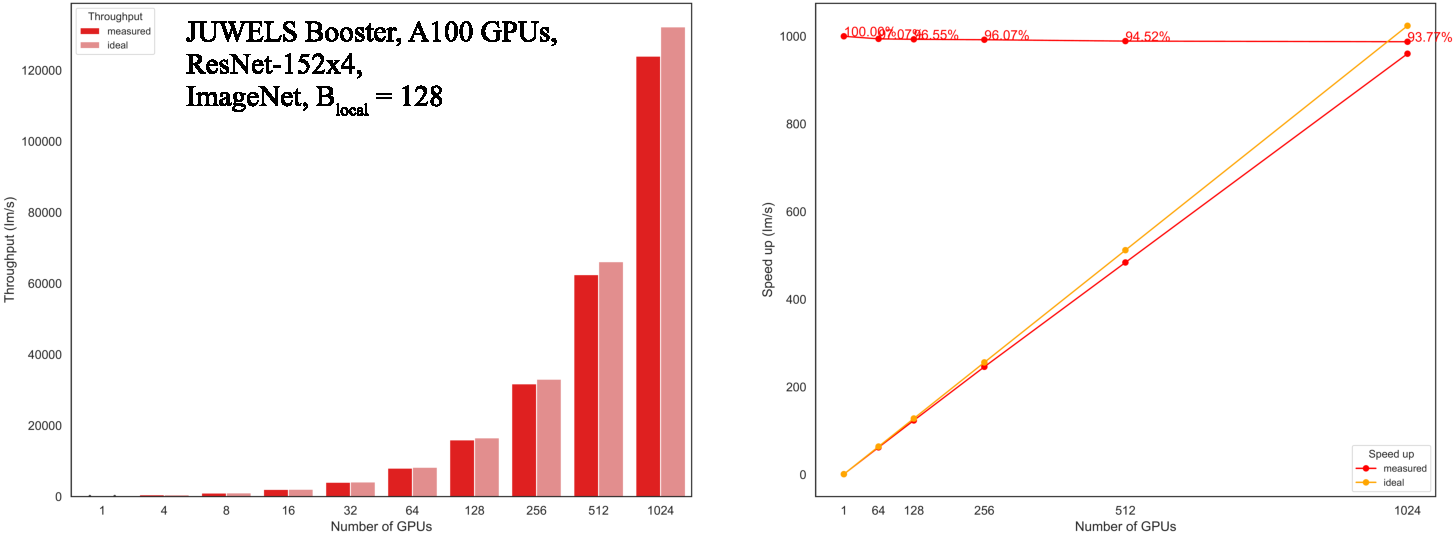
\includegraphics[width=0.9\textwidth]{../images/JUWELS_Booster_Ims_SpeedUp_ResNet-152x4_mod.pdf}}

\footnote<.->{\tiny Cherti and Jitsev, arXiv:2106.00116, MedNeurIPS
  Workshop, 2021}
\end{frame}

\begin{frame}{Distributed Training on ImageNet}
\protect\hypertarget{distributed-training-on-imagenet-5}{}
\begin{itemize}
\tightlist
\item
  Efficient distributed training in data parallel mode

  \begin{itemize}
  \tightlist
  \item
    requires good scaling of throughput Images/sec during training
  \end{itemize}
\end{itemize}

\center{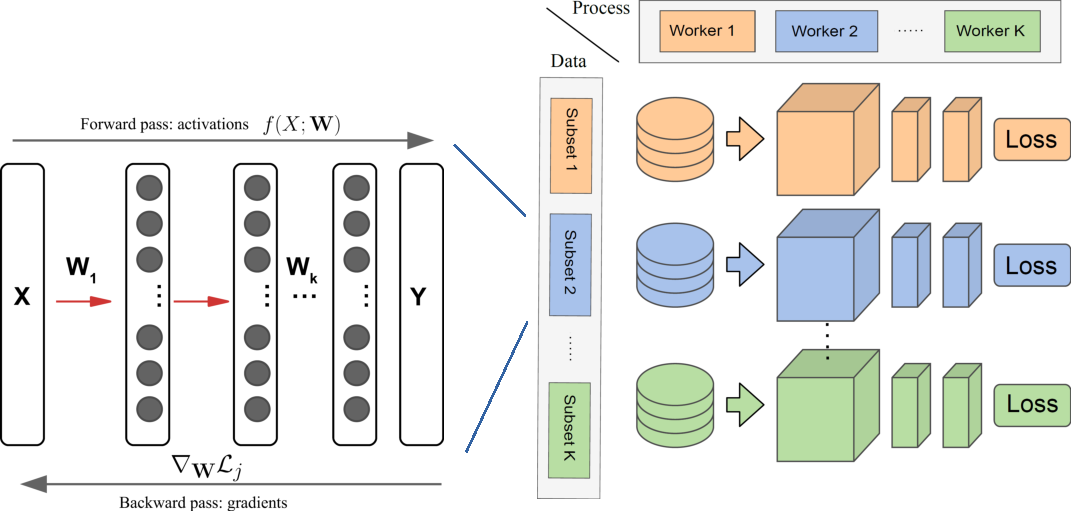
\includegraphics[width=0.9\textwidth]{../images/Data_Parallel_Model_Workers_Processes_Data_Subsets.pdf}}
\end{frame}

\begin{frame}[fragile]{Distributed Training on ImageNet}
\protect\hypertarget{distributed-training-on-imagenet-6}{}
\begin{itemize}
\tightlist
\item
  Efficient distributed training in data parallel mode
\end{itemize}

\begin{block}{Data IO}
\protect\hypertarget{data-io}{}
\begin{itemize}
\tightlist
\item
  Efficient file system, efficient data container

  \begin{itemize}
  \tightlist
  \item
    few separate large files; \textbf{sequential access}
  \item
    LMDB, HDF5, TFRecords, WebDataset
  \end{itemize}
\item
  Efficient Data pipeline

  \begin{itemize}
  \tightlist
  \item
    eg tf.data : interleave, cache, prefetch, \ldots{}
  \item
    avoid GPU starvation
  \end{itemize}
\end{itemize}
\end{block}

\begin{lstlisting}
...

141M /p/largedata/cstdl/ImageNet/imagenet-processed/train-00171-of-01024
137M /p/largedata/cstdl/ImageNet/imagenet-processed/train-00172-of-01024
139M /p/largedata/cstdl/ImageNet/imagenet-processed/train-00173-of-01024
142M /p/largedata/cstdl/ImageNet/imagenet-processed/train-00174-of-01024

...
\end{lstlisting}
\end{frame}

\begin{frame}{Distributed Training on ImageNet}
\protect\hypertarget{distributed-training-on-imagenet-7}{}
\begin{itemize}
\tightlist
\item
  Efficient distributed training in data parallel mode

  \begin{itemize}
  \tightlist
  \item
    requires efficient balance of GPU gradient compute and communication
  \end{itemize}
\end{itemize}

\center{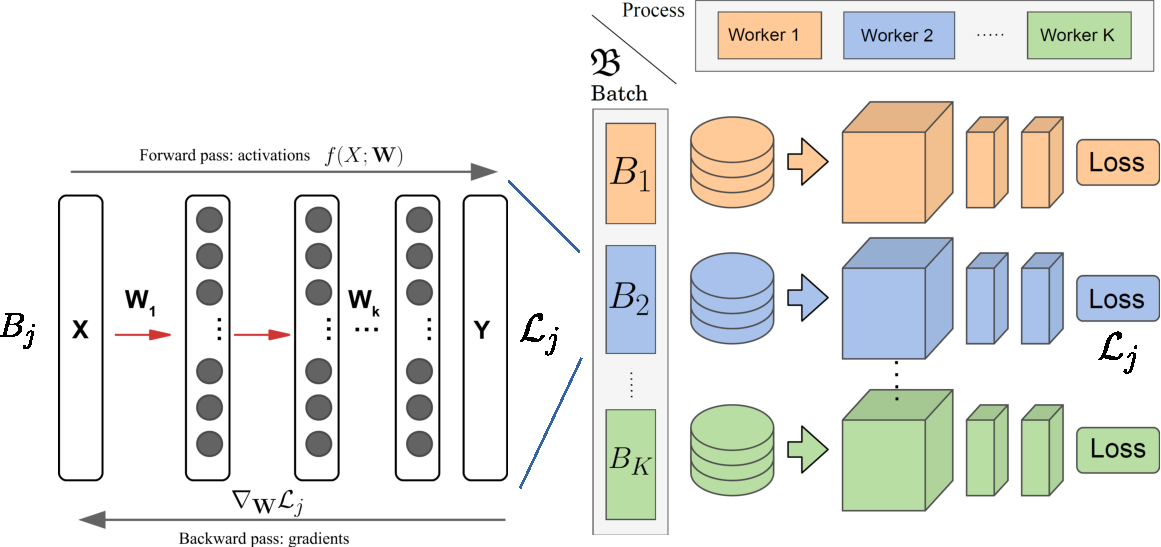
\includegraphics[width=0.9\textwidth]{../images/Forward_Backward_Data_Parallel_Workers_Batches.pdf}}
\end{frame}

\begin{frame}{Distributed Training on ImageNet}
\protect\hypertarget{distributed-training-on-imagenet-8}{}
\begin{itemize}
\tightlist
\item
  Efficient distributed training in data parallel mode
\end{itemize}

\begin{block}{SGD Optimization}
\protect\hypertarget{sgd-optimization}{}
\begin{itemize}
\tightlist
\item
  Corresponds to training single model with a larger effective batch
  size \(\vert \mathfrak{B} \vert = K \cdot \vert B_{\text{ref}} \vert\)

  \begin{itemize}
  \tightlist
  \item
    Image Throughput ideally increasing as
    \(\tau_K^{\*} = K \cdot \tau_{ref}\) Images/sec
  \end{itemize}
\item
  Make sure model fits into GPU memory

  \begin{itemize}
  \tightlist
  \item
    remember: this also depends on worker's batch size
    \(\vert B_{\text{ref}} \vert\) and input image resolution
  \end{itemize}
\item
  Avoid internode communication overhead \& bottlenecks

  \begin{itemize}
  \tightlist
  \item
    Most compute for forward-backward passes
  \item
    \(\vert B_{\text{ref}} \vert\) per GPU not too small
  \item
    High capacity network: InfiniBand
  \item
    Horovod: additional mechanisms, eg. Tensor Fusion
  \end{itemize}
\end{itemize}
\end{block}
\end{frame}

\begin{frame}{Distributed Training on ImageNet}
\protect\hypertarget{distributed-training-on-imagenet-9}{}
\begin{itemize}
\tightlist
\item
  ResNet-50 : efficient distributed training in data parallel mode on
  ImageNet-1k
\item
  Ultimate aim: reducing training \textbf{time to accuracy}

  \begin{itemize}
  \tightlist
  \item
    increasing throughput Images/sec during training only intermediate
    station!
  \item
    necessary, but not sufficient condition for speeding up model
    training
  \end{itemize}
\end{itemize}

\center{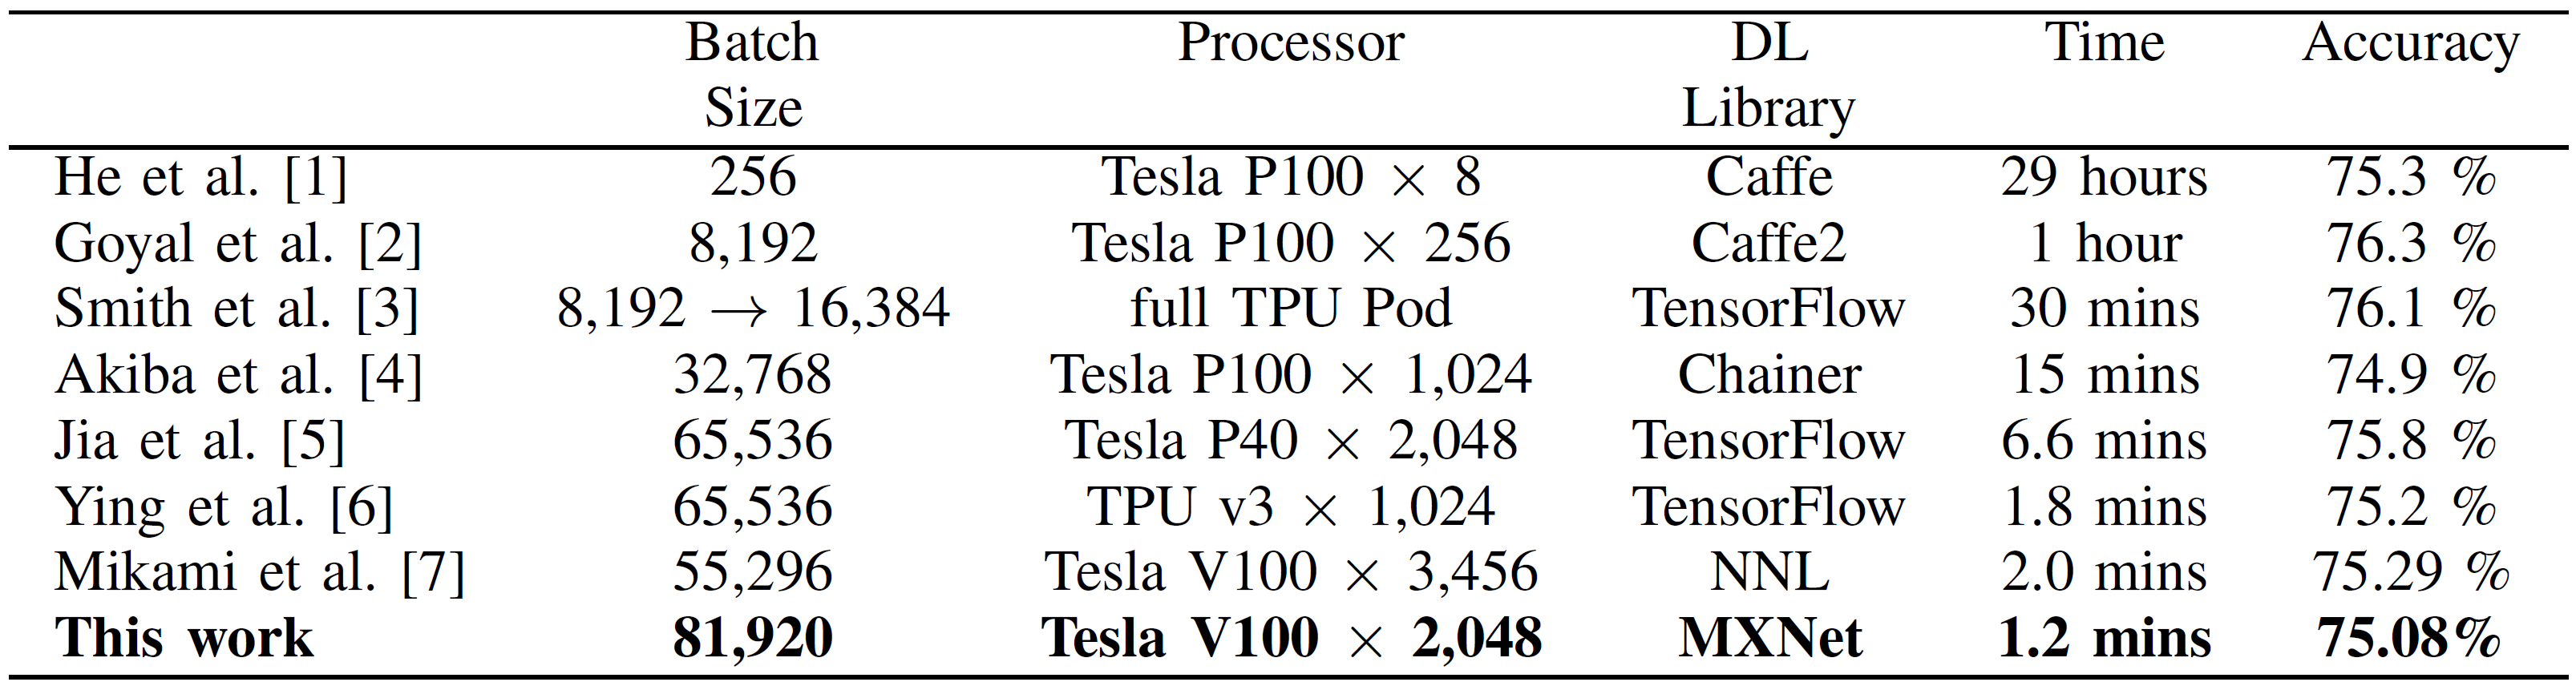
\includegraphics[width=0.8\textwidth]{../images/Yamazaki_RunTime_Table_ImageNet_ResNet-50_Accuracies.png}}

\vspace*{-1cm}

\footnote<.->{\tiny Yamazoto et al, 2019}
\end{frame}

\begin{frame}{Distributed Training on ImageNet}
\protect\hypertarget{distributed-training-on-imagenet-10}{}
\begin{block}{SGD Optimization}
\protect\hypertarget{sgd-optimization-1}{}
\begin{itemize}
\tightlist
\item
  Large effective batch size \(\vert \mathfrak{B} \vert\) may require
  hyperparameter retuning

  \begin{itemize}
  \tightlist
  \item
    Reminder: Large effective batch sizes alter optimization
  \end{itemize}
\end{itemize}
\end{block}

\center{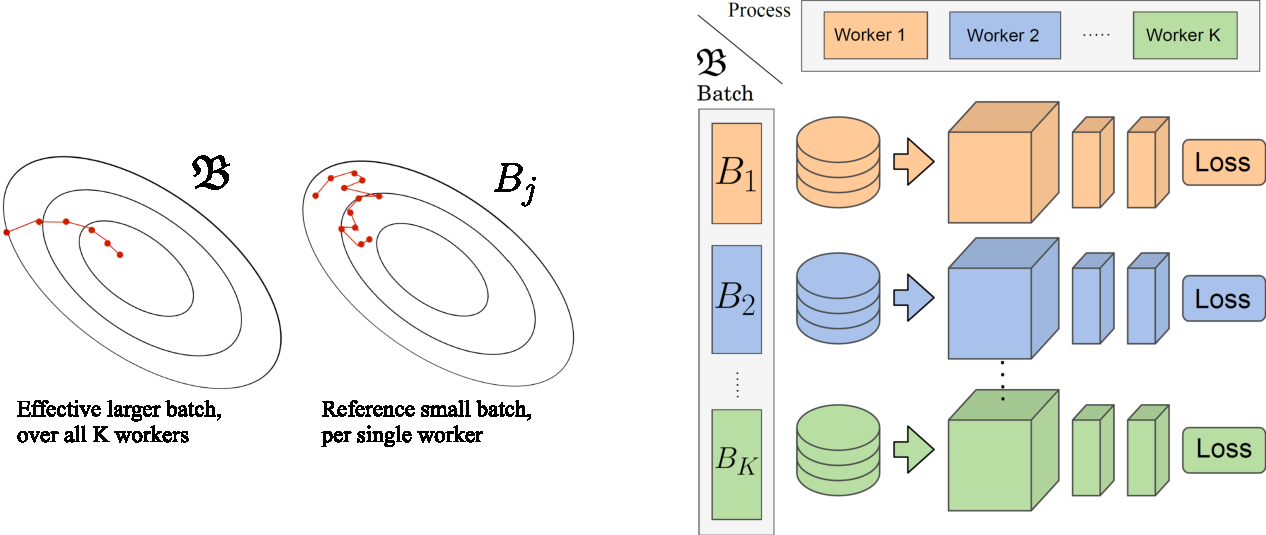
\includegraphics[width=0.9\textwidth]{../images/Large_Small_Reference_Batch_Data_Parallel_Model_Workers_Processes.pdf}}
\end{frame}

\begin{frame}{Distributed Training on ImageNet}
\protect\hypertarget{distributed-training-on-imagenet-11}{}
\begin{itemize}
\tightlist
\item
  Efficient distributed training in data parallel mode
\item
  Large effective batch sizes may require hyperparameter re-tuning

  \begin{itemize}
  \tightlist
  \item
    learning rate and schedule
  \item
    optimizer type
  \end{itemize}
\item
  Reminder: hyperparameter tuning for a given
  \(\vert \mathfrak{B} \vert\) - on the validation set!
\end{itemize}

\center{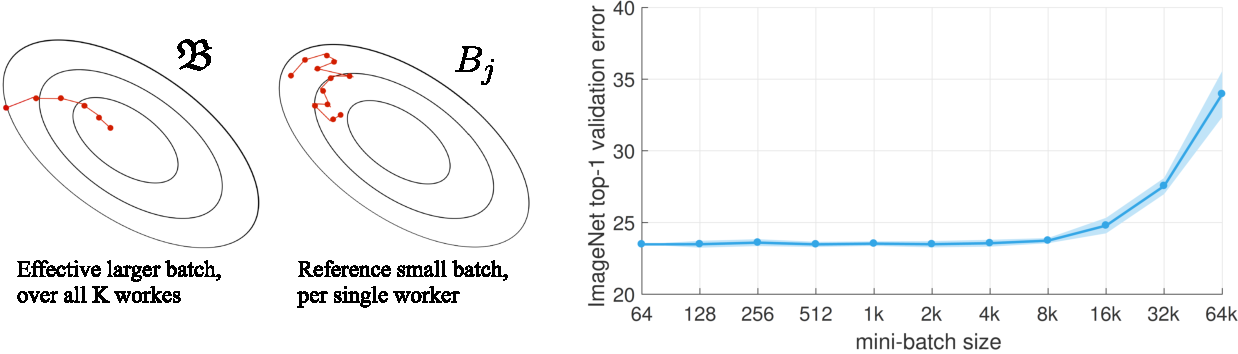
\includegraphics[width=0.8\textwidth]{../images/Effective_Reference_Batch_ImageNet_Goyal_2.pdf}}

\footnote<.->{\tiny Goyal et al, 2017}
\end{frame}

\begin{frame}{Distributed Training on ImageNet}
\protect\hypertarget{distributed-training-on-imagenet-12}{}
\begin{itemize}
\tightlist
\item
  Efficient distributed training in data parallel mode

  \begin{itemize}
  \tightlist
  \item
    Outlook: coping with training on large effective batch sizes
  \item
    Reducing training \textbf{time to accuracy}
  \end{itemize}
\end{itemize}

\center{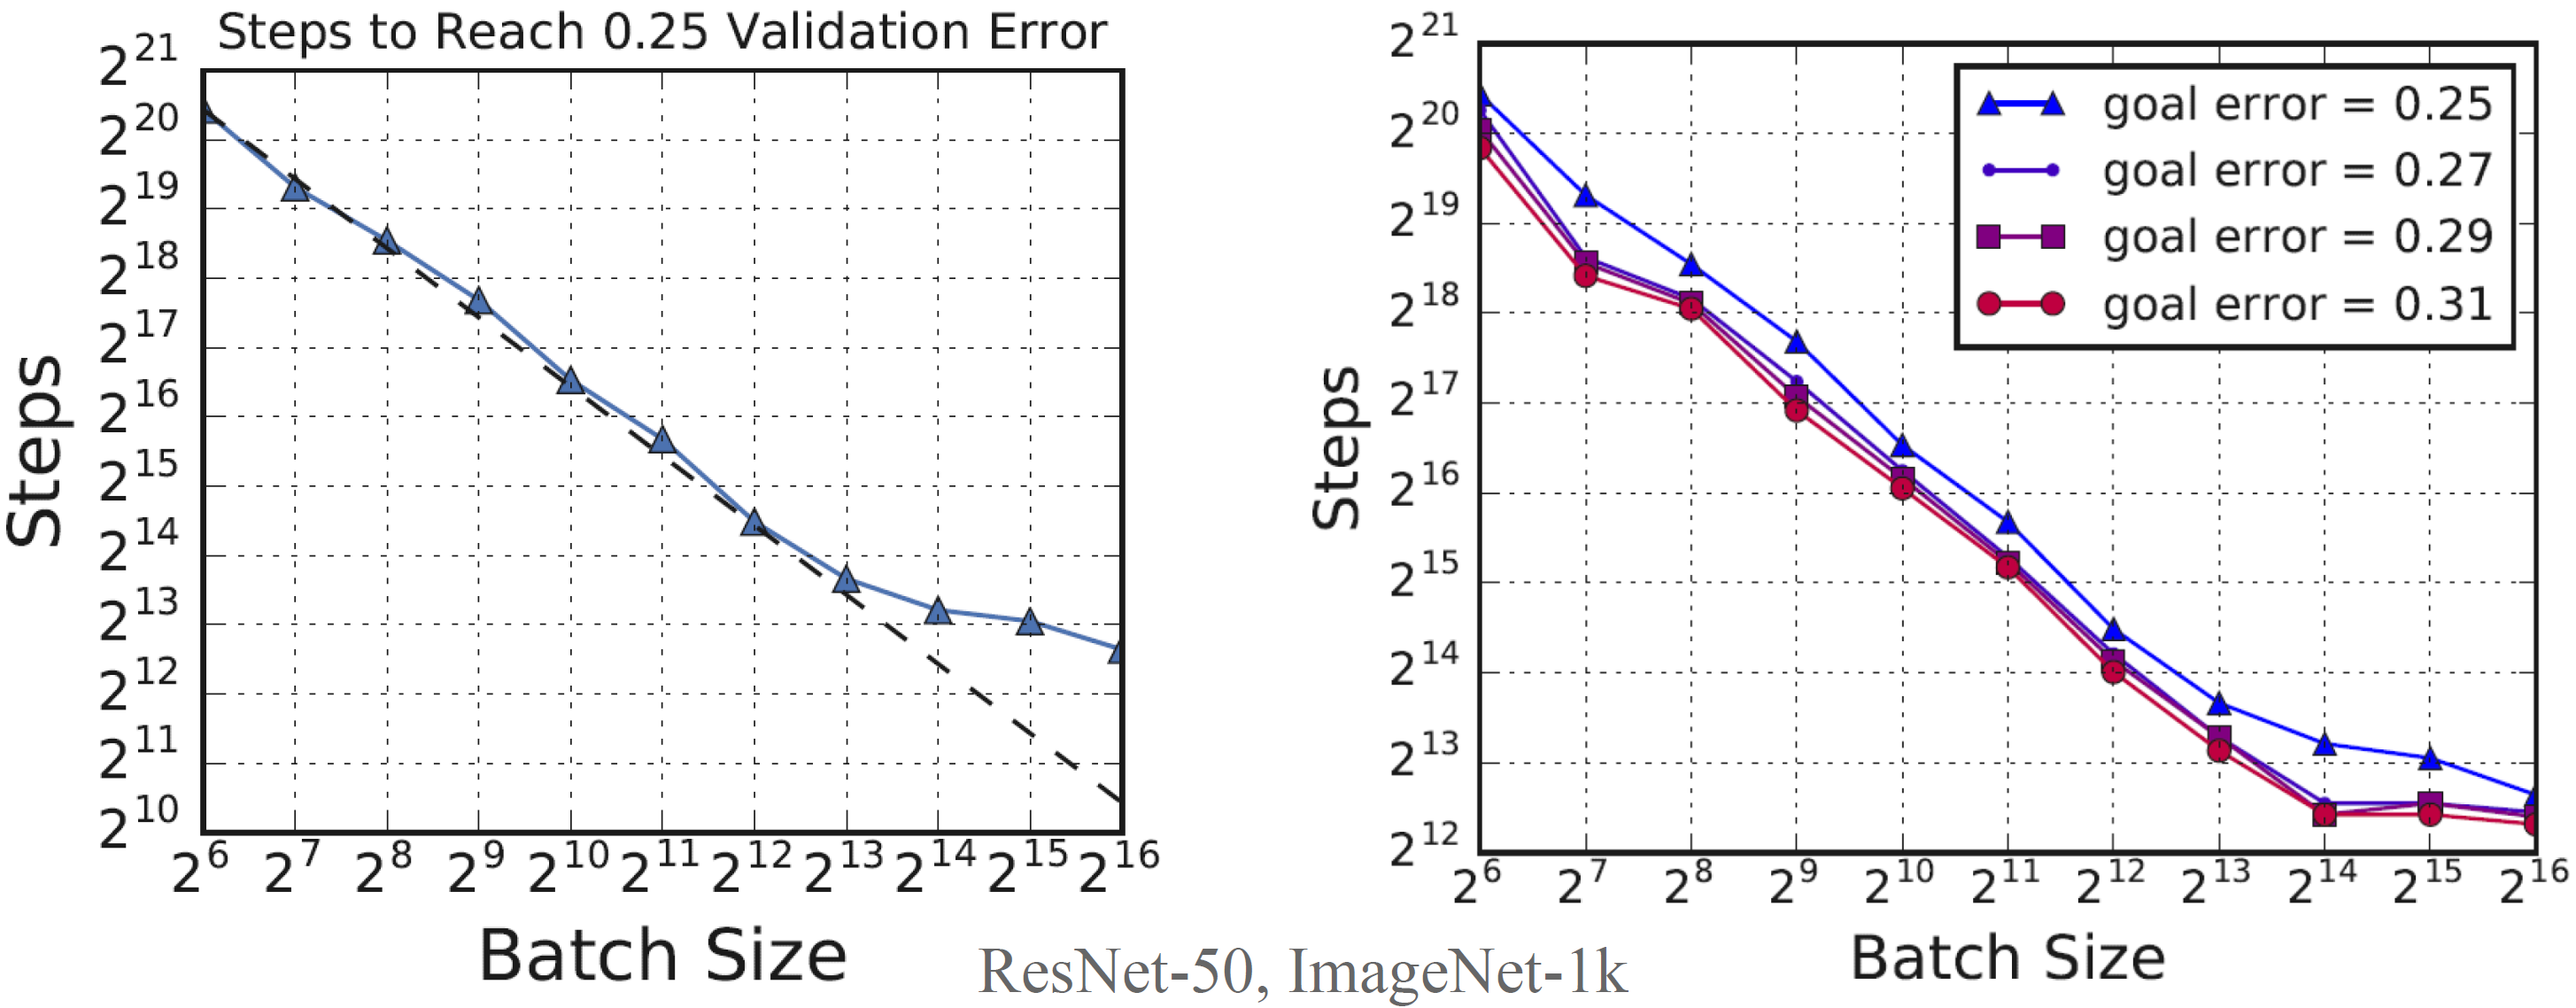
\includegraphics[width=0.8\textwidth]{../images/Batch_Size_Critical_ImageNet_ResNet-50_Goal_Error.png}}

\footnote<.->{\tiny Shallue et al, JMLR, 2019}
\end{frame}

\begin{frame}{Large Models, Large Data}
\protect\hypertarget{large-models-large-data}{}
\begin{block}{Summary}
\protect\hypertarget{summary-1}{}
\begin{itemize}
\tightlist
\item
  Reconciling generalization: large models generalize better

  \begin{itemize}
  \tightlist
  \item
    given enough data and compute to train
  \end{itemize}
\item
  Efficient data parallel training on large datasets like ImageNet-1k :
  possible
\item
  Data pipelines, high bandwidth \& low latency (eg InfiniBand), large
  batch sizes pave the way
\item
  Implementation of efficient distributed training: Horovod, PyTorch
  DDP, \ldots{}
\item
  Measures to stabilize training with large batches - upcoming lectures
\end{itemize}
\end{block}

\center{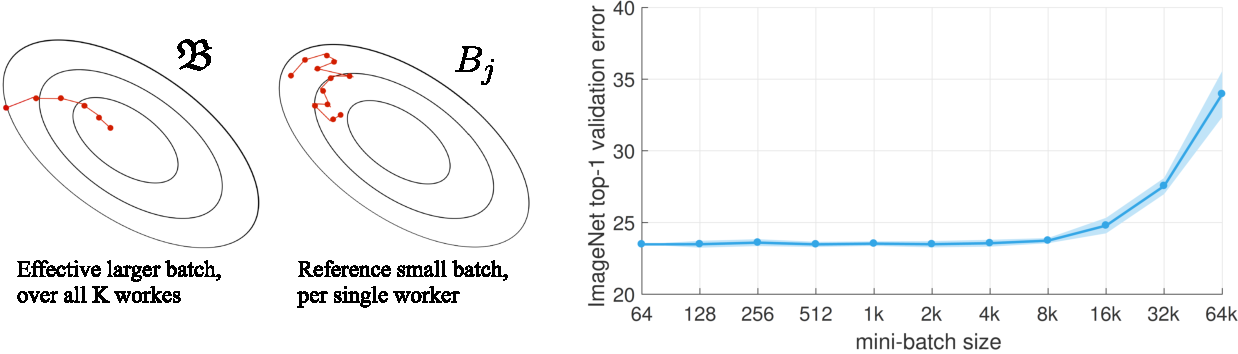
\includegraphics[width=0.8\textwidth]{../images/Effective_Reference_Batch_ImageNet_Goyal_2.pdf}}
\end{frame}
